%%%%%%%%%%%%%%
%% Run LaTeX on this file several times to get Table of Contents,
%% cross-references, and citations.

%% If you have font problems, you may edit the w-bookps.sty file
%% to customize the font names to match those on your system.

%% w-bksamp.tex. Current Version: Feb 16, 2012
%%%%%%%%%%%%%%%%%%%%%%%%%%%%%%%%%%%%%%%%%%%%%%%%%%%%%%%%%%%%%%%%
%
%  Sample file for
%  Wiley Book Style, Design No.: SD 001B, 7x10
%  Wiley Book Style, Design No.: SD 004B, 6x9
%
%
%  Prepared by Amy Hendrickson, TeXnology Inc.
%  http://www.texnology.com
%%%%%%%%%%%%%%%%%%%%%%%%%%%%%%%%%%%%%%%%%%%%%%%%%%%%%%%%%%%%%%%%

%%%%%%%%%%%%%
% 7x10
%\documentclass{wileySev}

% 6x9
\documentclass{wileySix}
\UseRawInputEncoding
\usepackage{graphicx}
\usepackage{listings}
\usepackage{float}
\usepackage{indentfirst}

\usepackage[T1]{fontenc}
\usepackage{inconsolata}

\usepackage{color}
\usepackage[table,xcdraw]{xcolor}


\definecolor{codegreen}{rgb}{0,0.6,0}
\definecolor{codegray}{rgb}{0.5,0.5,0.5}
\definecolor{codepurple}{rgb}{0.58,0,0.82}
\definecolor{backcolour}{rgb}{0.95,0.95,0.92}

\definecolor{pblue}{rgb}{0.13,0.13,1}
\definecolor{pgreen}{rgb}{0,0.5,0}
\definecolor{pred}{rgb}{0.9,0,0}
\definecolor{pgrey}{rgb}{0.46,0.45,0.48}
 
\lstdefinestyle{aing}{
    language=Java,
    captionpos=b,
    keepspaces=true,
    showspaces=false,
    showtabs=false,
    tabsize=2,
    numbers=left,
    numbersep=5pt,
    breaklines=true,
    showstringspaces=false,
    breakatwhitespace=true,
    backgroundcolor=\color{backcolour},
    commentstyle=\color{pgreen},
    keywordstyle=\color{pblue},
    stringstyle=\color{pred},
    numberstyle=\tiny\color{codegray},
    basicstyle=\footnotesize,
    moredelim=[il][\textcolor{pgrey}]{$$},
    moredelim=[is][\textcolor{pgrey}]{\%\%}{\%\%}
}


 \lstset{style=aing}

%%%%%%%
%% for times math: However, this package disables bold math (!)
%% \mathbf{x} will still work, but you will not have bold math
%% in section heads or chapter titles. If you don't use math
%% in those environments, mathptmx might be a good choice.

% \usepackage{mathptmx}

% For PostScript text
\usepackage{w-bookps}

%%%%%%%%%%%%%%%%%%%%%%%%%%%%%%%%%%%%%%%%%%%%%%%%%%%%%%%%%%%%%%%%
%% Other packages you might want to use:

% for chapter bibliography made with BibTeX
% \usepackage{chapterbib}

% for multiple indices
% \usepackage{multind}

% for answers to problems
% \usepackage{answers}

%%%%%%%%%%%%%%%%%%%%%%%%%%%%%%
%% Change options here if you want:
%%
%% How many levels of section head would you like numbered?
%% 0= no section numbers, 1= section, 2= subsection, 3= subsubsection
%%==>>
\setcounter{secnumdepth}{3}

%% How many levels of section head would you like to appear in the
%% Table of Contents?
%% 0= chapter titles, 1= section titles, 2= subsection titles, 
%% 3= subsubsection titles.
%%==>>
\setcounter{tocdepth}{2}

%% Cropmarks? good for final page makeup
%% \docropmarks

%%%%%%%%%%%%%%%%%%%%%%%%%%%%%%
%
% DRAFT
%
% Uncomment to get double spacing between lines, current date and time
% printed at bottom of page.
% \draft
% (If you want to keep tables from becoming double spaced also uncomment
% this):
% \renewcommand{\arraystretch}{0.6}
%%%%%%%%%%%%%%%%%%%%%%%%%%%%%%

%%%%%%% Demo of section head containing sample macro:
%% To get a macro to expand correctly in a section head, with upper and
%% lower case math, put the definition and set the box 
%% before \begin{document}, so that when it appears in the 
%% table of contents it will also work:

\newcommand{\VT}[1]{\ensuremath{{V_{T#1}}}}

%% use a box to expand the macro before we put it into the section head:

\newbox\sectsavebox
\setbox\sectsavebox=\hbox{\boldmath\VT{xyz}}

%%%%%%%%%%%%%%%%% End Demo


\begin{document}


\booktitle{APLIKASI QEUANGANS}
\subtitle{Dengan Android}

\authors{Faris Muhammad Ihsan, Syabriena Putri Veriane\\
\affil{Politeknik Pos Indonesia}
%Floyd J. Fowler, Jr.\\
%\affil{University of New Mexico}
}

\offprintinfo{Cerdas Menguasai Git, First Edition}{Rolly M. Awangga}

%% Can use \\ if title, and edition are too wide, ie,
%% \offprintinfo{Survey Methodology,\\ Second Edition}{Robert M. Groves}

%%%%%%%%%%%%%%%%%%%%%%%%%%%%%%
%% 
\halftitlepage

\titlepage


\begin{copyrightpage}{2019}
%Survey Methodology / Robert M. Groves . . . [et al.].
%\       p. cm.---(Wiley series in survey methodology)
%\    ``Wiley-Interscience."
%\    Includes bibliographical references and index.
%\    ISBN 0-471-48348-6 (pbk.)
%\    1. Surveys---Methodology.  2. Social 
%\  sciences---Research---Statistical methods.  I. Groves, Robert M.  II. %
%Series.\\
%
%HA31.2.S873 2007
%001.4'33---dc22                                             2004044064
\end{copyrightpage}

\dedication{`Jika Kamu tidak dapat menahan lelahnya belajar, 
Maka kamu harus sanggup menahan perihnya Kebodohan.'
~Imam Syafi'i~}

\begin{contributors}
\name{Rolly Maulana Awangga,} Informatics Research Center., Politeknik Pos Indonesia, Bandung,
Indonesia



\end{contributors}

\contentsinbrief
\tableofcontents
\listoffigures
\listoftables
\lstlistoflistings


\begin{foreword}
Sepatah kata dari Kaprodi, Kabag Kemahasiswaan dan Mahasiswa
\end{foreword}

\begin{preface}
Buku ini diciptakan bagi yang awam dengan git sekalipun.

\prefaceauthor{R. M. Awangga}
\where{Bandung, Jawa Barat\\
Februari, 2019}
\end{preface}


\begin{acknowledgments}
Terima kasih atas semua masukan dari para mahasiswa agar bisa membuat buku ini 
lebih baik dan lebih mudah dimengerti.

Terima kasih ini juga ditujukan khusus untuk team IRC yang 
telah fokus untuk belajar dan memahami bagaimana buku ini mendampingi proses 
Intership.
\authorinitials{R. M. A.}
\end{acknowledgments}

\begin{acronyms}
\acro{3GP}{3gpp}
\acro{3GPP}{3rd Generation Partnership Project}
\acro{A2DP}{Advance Audio Distribution Profile}
\acro{API}{Application Programing Interface}
\acro{ASF}{Apache Software Foundation}
\acro{AVRCP}{Audio / Video Remote Control Profile}
\acro{C2DM}{Android Cloud to Device Messaging}
\acro{CDMA}{Code-Vision Multiple Access}
\acro{E-MAIL}{Electronic Mail}
\acro{EVDO}{Evolution-Data Optimized}
\acro{G-MAIL}{Google Mail}
\acro{HP}{Handphone}
\acro{HTML}{Hypertext Markup Language}
\acro{IMAP}{Internet Message Access Protocol}
\acro{JIT}{Just-In-Time Manufacturing}
\acro{LED}{Light Emitting Diode}
\acro{MMS}{Multimedia Messaging Service}
\acro{MP4}{MPEG4}
\acro{MPEG}{Moving Picture Expert Group}
\acro{OEM}{Original Equipment Manufacturer}
\acro{OHA}{Open Handset Alliance}
\acro{OS}{Operating System}
\acro{POP3}{Post Office Protocol Version 3}
\acro{SMS}{Short Message Service}
\acro{SMTP}{Simmple Mail Transfer Protocol}
\acro{UI}{User Interface}
\acro{USB}{Universal Serial Bus}
\acro{WI-FI}{Wireless Fidelity}
\acro{WVGA}{Wide VGA}
\acro{VGA}{Video Graphics Array}
\acro{XHTML}{Extensible Hypertext Markup Language}
\end{acronyms}

\begin{glossary}
\term{git}Merupakan manajemen sumber kode yang dibuat oleh linus torvald.

\term{bash}Merupakan bahasa sistem operasi berbasiskan *NIX.

\term{linux}Sistem operasi berbasis sumber kode terbuka yang dibuat oleh Linus Torvald
\end{glossary}

\begin{symbols}
\term{A}Amplitude

\term{\hbox{\&}}Propositional logic symbol 

\term{a}Filter Coefficient

\bigskip

\term{\mathcal{B}}Number of Beats
\end{symbols}

\begin{introduction}

%% optional, but if you want to list author:

\introauthor{Rolly Maulana Awangga, S.T., M.T.}
{Informatics Research Center\\
Bandung, Jawa Barat, Indonesia}

Pada era disruptif  \index{disruptif}\index{disruptif!modern} 
saat ini. git merupakan sebuah kebutuhan dalam sebuah organisasi pengembangan perangkat lunak.
Buku ini diharapkan bisa menjadi penghantar para programmer, analis, IT Operation dan Project Manajer.
Dalam melakukan implementasi git pada diri dan organisasinya.

Rumusnya cuman sebagai contoh aja biar keren\cite{awangga2018sampeu} \cite{maulani2018analysis}.

\begin{equation}
ABC {\cal DEF} \alpha\beta\Gamma\Delta\sum^{abc}_{def}
\end{equation}

\end{introduction}

%%%%%%%%%%%%%%%%%%Isi Buku_
\chapter{Sejarah Android}
\section{Sejarah Android}

\begin{figure}[H]
    \centering
    
\includegraphics[scale=0.2]{pictures/logo_android.jpg}
    \caption{Logo Android}
\end{figure}

Android adalah sistem operasi dengan basis linux yang dirancang untuk perangkat yang bergerak atau layar sentuh \textit{touchscreen} seperti telepon pintar \textit{smartphone} dan \textit{tablet}. Android merupakan sistem operasi \textit{open source} (aplikasi yang tidak dipegang hanya untuk seorang saja tetapi orang lain bisa menggunakan \textit{sourcecode} tersebut). Android ini mengunakan lisensi dari Google yang kodenya tersebut berada dibawah Lisensi \textit{Apache}. Lisensi \textit{Apache} merupakan lisensi yang bebas untuk \textit{software} yang ditulis oleh \textit{Apache Software Foundation} (ASF).

Android berdiri pada bulan Oktober 1980, tepatnya di Palo Alto,  California. Android ini didirikan oleh Andy Rubin, Rich Muner, Nick Sears, dan Chris White. Android dikembangkan oleh perusahaan dengan nama \textit{Ancroid.inc}. Pada tahun 2005 perusahaan tersebut mendapatkan dukungan finansial dari \textit{google.inc}

Pada awalnya Android tidak dibbuat untuk ponsel, namun android pertama kali dibuat untuk kamera digital. Tetapi, dengan melihat peluang yang lebih besar jika Android digunakan untuk perangkat \textit{mobile}, maka Android digunakan pada perangkat \textit{mobile} yang ditujukan untuk menyaingi \textit{Symbian} dan \textit{Windows Mobile}.

Secara resmi, Android dirilis pada tahun 2007 bersamaan dengan berdirinya \textit{Open Handset Alliance}. \textit{Open Handset Alliance} merupakan \textit{Open Source Developer} bagi perangkat \textit{mobile} atau seluler. Tahun 2008, \textit{Handphone} pertama yang menggunakan sistem operasi android kemudian dirilis, \textit{handphone} ini bernama \textit{HTC Dream}. Dua tahun setelah perilisan \textit{Handphone} ini, Google menyusul dengan merilis \textit{Smartphone} dengan seri \textit{Nexus One} yang proses pembuatannya dibantu oleh \textit{HTC}. Dengan dirilisnya \textit{Handphone} tersebut, memancing kemunculan-kemunculan berbagai brand dari \textit{OEM} yang bermacam-macam. Dimulai dari \textit{Samsung, Lenovo, HTC, ASUS, LG} dan masih banyak lagi.

\begin{figure}[!htbp]
    \centering
    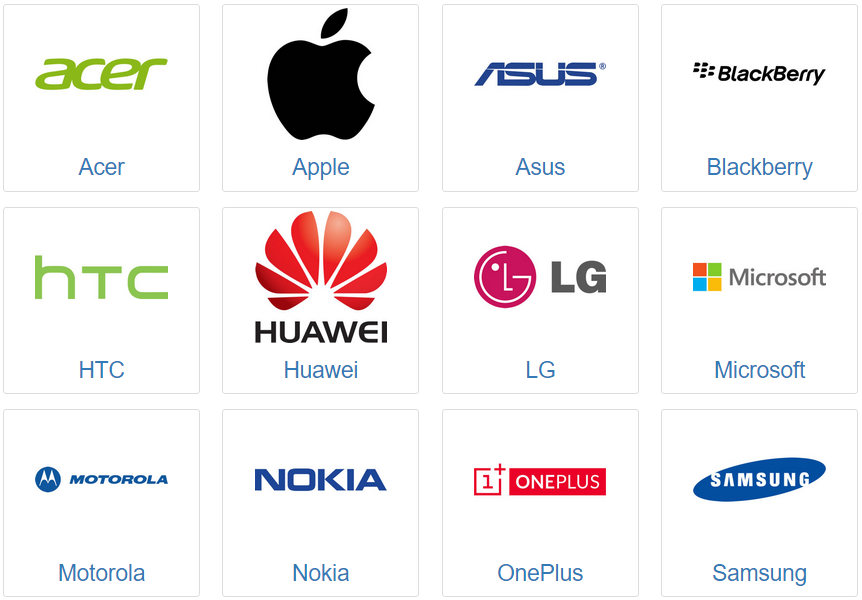
\includegraphics[scale = 0.3]{pictures/merk-OEM-Android.png}
    \caption{OEM Android Smartphone}
\end{figure}

Selain berfokus pada \textit{smartphone}, Google juga banyak mengembangkan aplikasi Android untuk perangkay lainnya. Contohnya Google mengembangkan Android TV yang digunakan untuk televisi, Android Auto yang digunakan pada, dan Android Wear pada jam tangan. Aplikasi android tersebut memiliki \textit{Interface} yang berbeda beda sesuai dengan kebutuhan dan fungsionalitasnya masing-masing. 

\textit{Open Source Code} dan lisensi yang diguakan pada Android tentunya dapat membuat Sistem Operasi ini dapat diubah-ubah dan dimodifikasi dengan bebas yang kemudian dapat di distribusikan oleh para \textit{developer} Android itu sendiri. Selain mudah untuk digunakan, Android memiliki \textit{Developer Community} (Komunitas Pengembang) sendiri yang dapat memperluas fungsionalitas dari perangkat yang umumnya digunakan menggunakan bahasa pemrograman \textit{Java}. Selain \textit{java}, Android ini juga dapat menggunakan bahasa pemrograman \textit{Kotlin}. Lebih dari Satu juta aplikasi kemudian tersedia untuk android, dan miliaran aplikasi telah melakukan di\textit{download} dari \textit{Google Play} (toko utama yang berisi aplikasi-aplikasi dari Android)

Dimulai sejak tahun 2008, Android melakukan pembaruan untuk meningkatkan kinerja aplikasinya secara bertahap dengan cara menambahkan fitur-fitur yang baru dan memperbaiki \textit{error} dan \textit{bug} yang terdapat pada produk dengan versi yang sebelumnya. Setiap versi dari android biasanya disusun dengan nama alfabetis dan nama yang digunakan adalah nama makanan-makanan yang ringan atau cemilan. Sebagai contoh pada android versi 7.0 yang diberi nama Android \textit{Nougat}, Kemudian Android 8.0 yang diberi nama \textit{Oreo} dan seterusnya. 

\section{Versi Pada Android}
Pada awal kemunculan Android, Android telah mengeluarkan banyak versi. Setiap versi dari android ini tentunya memiliki fitur-fiturnya masing-masing sesuai dengan perkembangan zaman. Hal ini tentunya sebagai cara agar mengalahkan pesaingnya yang menggunakan OS yang lainnya seperti Apple iOS, Windows, Blackberry, Symbian dan lainnya. 
\begin{enumerate}

\item Android 1.0 \textbf{Apple Pie}\\
\begin{figure}[!htbp]
    \centering
    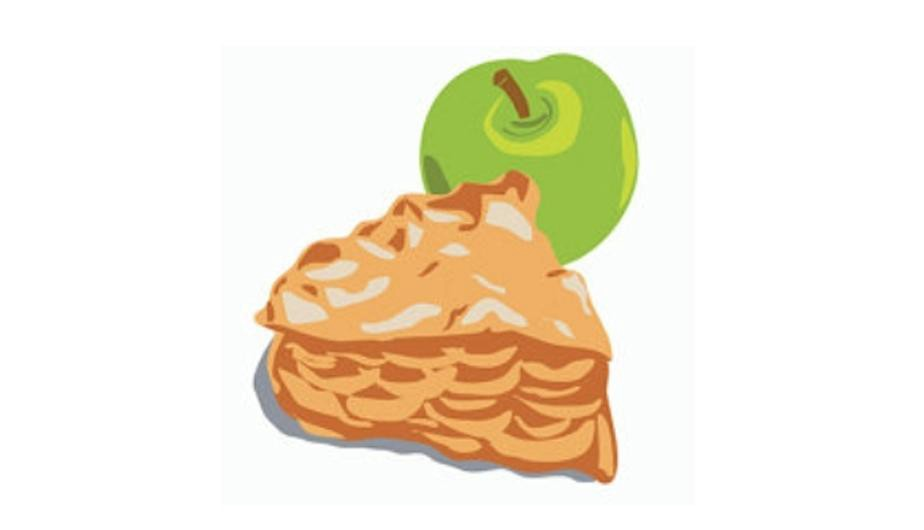
\includegraphics[scale = 0.3]{pictures/android-apple-pie.jpg}
    \caption{Android Apple Pie}
    \label{}
\end{figure}

Android versi pertama ini merupakan android dengan versi 1.0 yang diberi nama Android \textit{Apple Pie} yang dirilis oleh android  pada 23 September 2008 dan hanya memiliki fitur yang terbatas. Fitur fitur tersebut adalah:

\begin{enumerate}
    \item \textit{Play Store}
    \item Kamera
    \item \textit{Web Browser}
    \item \textit{G-Mail Sychronization}
    \item Kontak
    \item Google Agenda
    \item Google \textit{Maps}
\end{enumerate}
Selain itu, Android versi ini juga sudah mendukung fasilitas youtube. Setidaknya Google dan OHA telas merilis 2 versi saat sebelum Android beta yang dirilis pada bulan November 2007. Pada Android Versi Alpha memiliki sebutan atau \textit{codename} \textit{Astro Boy, Bender,} dan R2-D2.\\

KELEBIHAN
\begin{enumerate}

\item Android Market\\ 
Android market merupakan aplikasi untuk \textit{mendownload} dan \textit{mengupdate} aplikasi yang terinstall melalui toko resmi dari Android.
\item \textit{Web Browser}\\
Android \textit{Web Browser} merupakan aplikasi untuk \textit{searching website}, menampilkan halaman \textit{Web HTML} dan \textit{XHTML} dan dapat digunakan untuk melihat halaman web dengan \textit{fullscreen} dan dapat juga diperbesar.
untuk menampilkan, memperbesar dan melihat dalam layar penuh halaman \textit{Web HTML} dan \textit{XHTML}
\item Kamera
\item Memungkinkan pengelompokan ikon-ikon aplikasi ke dalam satu folder pada bagian layar utama (\textit{homescreen}).
\item Dapat memiliki dan mengakses \textit{E-Mail}, mendukung fasilitas POP3, IMAP4, dan SMTP
\item Sinkronisasi \textit{G-mail} dengan menggunakan aplikasi \textit{G-mail}.
\item Sinkronisasi \textit{Google Contacts} dengan menggunakan aplikasi \textit{People}.
\item Sinkronisasi \textit{Google Calendar} dengan menggunakan aplikasi \textit{Calendar}.
\item Aplikasi \textit{Google Maps} \\
Aplikasi \textit{Google Maps} ini menyediakan informasi mengenai Latitude, derdapat fitur \textit{Street View}, dapat melihat melihat peta dan tampilan melalui citra satelit, menemukan lokasi yang akan dituju dan dapat memberi petunjuk arah saat mengemudi kendaraan maupun saat berjalan-jalan.
\item \textit{Google Sync}\\ 
Fitur ini dapat memungkinkan pengelolaan sinkronisasi pada aplikasi \textit{Gmail, People, dan Calendar}.
\item Google Search\\
Fitur ini dapat memungkinkan pengguna untuk \textit{Searching} sesuatu menggunakan \textit{website}.
\item \textit{Google Talk} \\
\textit{Google Talk} merupakan sebuah aplikasi pesan instan yang diproduksi oleh google
\item Pesan instan, pesan teks (SMS), dan MMS.
\item \textit{Media Player}\\
\textit{Media Player}ini digunakan untuk mengelola, mengimpor, dan memutar file yang mendukung pada berkas penyimpanan. Tetapi, pada versi ini belum menyediakan dukungan \textit{Video} dan \textit{Bluetooth Stereo}
\item Notifikasi\\
Notifikasi ini merupakan fitur yang akan muncul pada status bar, dengan diberikan pilihan pengaturan untuk mengatur \textit{Ringtone}, cahaya \textit{LED} yang dikeluarkan maupun nada getar.
\item \textit{Voice Dialer}\\ 
\textit{Voice Dialer} ini memberikan akses kepada pengguna untuk memanggil kontak tanpa harus mengetikan nama ataupun nomor telepon orang yang akan dituju.
\item Wallpaper\\ 
Fitur ini dapat digunakan pengguna untuk mengatur gambar \textit{Wallpaper} pada \textit{Homescreen} perangkat android pengguna. 
\item \textit{Youtube Video Player}
\item Fitur Pendukung Lainnya seperti:
\begin{enumerate}
    \item Jam Alarm
    \item Kalkulator
    \item Panggilan
    \item \textit{Homescreen Launcher}
    \item Galeri
    \item Pengaturan
\end{enumerate}
\item Wi-Fi
\item Bluetooth\\
\end{enumerate}

KEKURANGAN
\begin{enumerate}
    \item Versi Android ini pada awalnya belum memiliki nama yang cocok sehingga tidak diberi nama dan hal tersebut dapat membuat bingung masyarakat karena tidak akan mudah untuk diingat.\\
\end{enumerate}


\item Android 1.1 \textbf{Banana Bread}\\
\begin{figure}[!htbp]
    \centering
    
\includegraphics[scale = 1.2]{pictures/android-banana-bread.jpg}
    \caption{Android Banana Bread}
    \label{}
\end{figure}

Pada Februari 2009, Android meng-\textit{upgrade} dari versi sebelumnya (versi 1.0) ke versi 1.1 yang bernama Android \textit{Banana Bread}. Fitur pada android ini tidak jauh bedanya dengan versi sebelumnya. \textit{Smartphone} pertama yang menggunakan versi ini adalah \textit{HTC}. Android 1.1 \textit{Banana Bread} ini memiliki nama lain yaitu \textit{"Petit Four"}. Nama ini tentunya bukan nama resmi yang dikeluarkan oleh pihak Android. Versi ini merupakan versi yang berkembang dan memperbaiki beberapa bug (\textit{Error}) yang ada pada Android sebelumnya. Versi ini juga mengubah \textit{API} dari android yang sebelumnya. Selain itu, Android ini menambahkan fitur fiitur baru yaitu:
\begin{enumerate}
    \item \textit{Maps} dan pencarian lokasi bisnis sudah terdapat rincian tempat.
    \item Tombol Panggilan yang dapat di sembunyikan atau di tampilkan.
    \item Dapat menyimpan lampiran dalam pesan
    \item Mendapat dukungan \textit{Marquee} pada ruang sistem.\\
\end{enumerate}


\item Android 1.5 \textbf{Cupcake}\\
\begin{figure}[!htbp]
    \centering
    
\includegraphics[scale = 0.3]{pictures/android-cupcake.jpg}
    \caption{Android Cupcake}
    \label{}
\end{figure}

Adroid Versi ini diluncurkan pada bulan April 2009 dan tidak memiliki perbedaan yang signifikan dengan versi Android yang terdahulu. Meski dengan sedikit perbedaan, android ini mendapatkan fitur tambahan seperti \textit{Support Bluetooth A2DP, AVRCP, Soft Keyboard} dengan \textit{Text Suggestion, Record} ataupun \textit{Watch Videos}. Android ini merupakan versi Android yang mulai menggunakan nama makanan cemilan yaitu "\textit{Cupcake}". Pada Android versi ini, terdapat pembaruan, penambahan fitur, dan Perubahan \textit{User Interfaces}, beberapa perubahannya yaitu:
\begin{enumerate}
    \item \textit{Third Party Virtual Keyboard} dengan prediksi teks dan \textit{User Dictionary}(Kamus pengguna)
    \item Mendapat dukungan \textit{Widget}
    \item Sudah memiliki kemampuan \textit{record video} dan memutar video dengan format MPRG-4 (.mp4) dan .3gp
    \item Memiliki fasilitas \textit{pairing bluetooth}
    \item Mendukung \textit{bluetooth stereo} \textit{A2DP dan AVRCP}
    \item Penambahan fitur \textit{Copy and Paste} pada \textit{Web Browser}
    \item Fitur Menambahkan foto pada kontak telepon
    \item Pada bagian panggilan, tanggal dan waktu ditampilkan di bagian log panggilan
    \item Dapat memanggil kontak melali log panggilan
    \item Animasi saat terjadi transisi layar
    \item Fitur \textit{Auto Rotate} (Putar Otomatis)
    \item Update Animasi saat \textit{Booting} OS 
    \item Dapat \textit{Upload} video ke youtube
    \item Dapat \textit{Upload} foto ke picasa\\
\end{enumerate}


\item Android 1.6 \textbf{Donut}\\
\begin{figure}[!htbp]
    \centering
    
\includegraphics[scale=0.5]{pictures/android_donut.jpg}
    \caption{Android Donut}
    \label{}
\end{figure}

Android Versi 1.6 atau dikenal dengan Android \textit{Donut} merupakan versi android yang dirilis pada tanggal 15 September 2009, dan terdapat fitur-fitur tambahan dari versi yang sebelumnya. Android ini memiliki sedikit kesalahan (bug atau \textit{error}) pada sistemnya. Selain itu, Android ini memiliki fitur yang cukup banyak yang ditambahkan oleh Google sehingga Android ini terbilang Android dengan versi yang cukup sempurna pada zamannya. Fitur-fitur tambahan pada Android versi ini adalah sebagai berikut:
\begin{enumerate}
    \item Terdapat fitur pencarian suara dan teks dalam \textit{history, bookmark,} kontak dan web.
    \item Fitur untuk menyertakan konten pada \textit{Developer} pada hasil pencarian.
    \item \textit{Voice machine} yang dapat mengucapkan berbagai bahasa dan membuat Android tertentu dapat mengucapkan teks.
    \item Pencarian menjadi lebih mudah
    \item Kemampuan untuk melihat sedikit cuplikan aplikasi di \textit{Android Market}
    \item Galeri, Kamera dan \textit{Video recorder} yang terintegrasi
    \item Akses Kamera lebih cepat
    \item Dapat memilih \textit{multifiles} untuk menghapus foto dalam sekala banyak.
    \item \textit{Update} pada teknologi \textit{CDMA/EVDO, 802.1x, VPN} dan mesin pengucap teks
    \item Mendukung resolusi layar \textit{WVGA}
    \item Peningkatan pencarian dan kamera
    \item Memperluas kerangka kerja, Gestur dan penambahan \textit{tools GestureBuilder Developer}.\\
\end{enumerate}

KEKURANGAN
\begin{enumerate}
    \item Hanya aplikasi tertentu yang dapat diinstall disini.
    \item Tidak ada \textit{equalizer} pada \textit{Music Player}nya.
    \item Android market tidak terintegrasi
    \item Keypad yang lambat
    \item \textit{Touch Responsiveness} kurang.\\
\end{enumerate}


\item Android 2.0 \textbf{Eclair}
\begin{figure}[!htbp]
    \centering
    
\includegraphics[scale=0.3]{pictures/android-eclair.jpg}
    \caption{Android Eclair}
    \label{}
\end{figure}

Android versi 2.0 ini bernama android \textit{eclair} yang dirilis pada tanggal 26 Oktober 2009. Android versi ini memiliki beberapa jenis \textit{API level} yaitu:
\begin{enumerate}
    \item Android Eclair 2.0 (API level 5)\\
    Android versi 2.0 ini dirilis pada tanggal 26 Oktober 2009. Pada Android versi ini memiliki beberapa fitur tambahan dari versi-versi sebelumnya. Perubahan fitur pada android versi ini adalah:
    \begin{enumerate}
        \item Bluetooth 2.1
        \item \textit{Multi-touch system}
        \item \textit{Live wallpaper}
        \item \textit{Flash} kamera, \textit{Digital Zoom, Skin mode, macro focus}
        \item HTML
        \item \textit{Digital Zoom}
        \item \textit{Support Microsoft Exchange}
        \item Update pada UI \textit{Web Browser} dengan fitur \textit{bookmark, double tap zoom, support HTML5}
        \item Multi akun pada saat sinkronisasi menggunakan \textit{E-Mail} dan kontak
        \item \textit{E-Mail} untuk \textit{Microsoft Exchange} dengan kemampuan untuk mencari \textit{E-Mail} dari beberapa akun dalam satu halaman
        \item Dapat memilih foto kontak
        \item Opsi untuk memanggil, mengirim sms dan \textit{E-Mail} pada kontak 
        \item Mampu mencari SMS dan MMS yang tersumpan. Pesan yang terlalu lama akan terhapus dengan sendirinya jika sudah mencapai batas maksimum.
        \item Kecepatan \textit{keyboard virtual} lebih cepat dan \textit{support} kamus yang mempelajari kata dan nama kontak
        \item Menyempurnakan UI dari kalender, menampilkan notifikasi kalender.
        \item Kecepatan \textit{Software} lebih optimal
        \item Resolusi layar lebih beragam
        \item \textit{Update google maps} ke versi 3.1.2
    \end{enumerate}
    
    \item Android Eclair 2.0.1 (API level 6)\\
    Android ini dirilis pada tanggal 3 Desember 2009. Versi ini merupakan \textit{update} dari versi sebelumnya (Android Eclair 2.0). \textit{Update} yang terdapat pada versi ini adalah:
    \begin{enumerate}
        \item Perubahan minor pada API nya
        \item Perbaikan pada bug yang terjadi di versi sebelumnya
        \item Perubahan \textit{workflow}(Kerangka kerja) pada sistemnya
    \end{enumerate}

    \item Android Eclair 2.1 (API level 7)\\
    Android ini dirilis pada tanggal 12 Januari 2010. Versi ini merupakan \textit{update} dari versi sebelumnya (Android Eclair 2.0.1). \textit{Update} yang terdapat pada versi ini adalah:
    \begin{enumerate}
        \item Perubahan Minor pada API nya
        \item Perbaikan pada bug yang terjadi di versi sebelumnya\\
    \end{enumerate}
\end{enumerate}

\item Android 2.2.9 \textbf{Froyo}\\
\begin{figure}[!htbp]
    \centering
    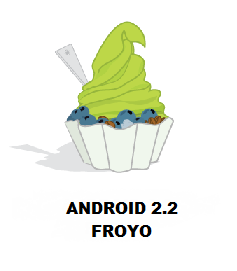
\includegraphics[scale = 0.45]{pictures/android-froyo.png}
    \caption{Android Froyo}
    \label{}
\end{figure}

Android 2.2.9 atau dikenal dengan nama android Froyo, diluncurkan pada Mei 2010. Versi ini dirilis oleh perusahaan besar yaitu Google. Versi ini merupakan versi penyempurna dari versi versi yang sebelumnya. Versi ini dibentuk dengan tujuan untuk meningkatkan kinerja dari sistem Android. Fitur fitur yang terdapat pada versi android ini adalah: 
\begin{enumerate}
    \item Peningkatan kecepatan sistem
    \item Pengimplementasian JIT
    \item Integrasi mesin dari JavaScript V8 Chrome kedalam \textit{Web Browser}
    \item Dukungan \textit{Android Cloud to Device Messaging (C2DM) }
    \item Meningkatkan \textit{Microsoft Exchange Support}, keamanan, pencarian otomatis, GAL, sinkronisasi pada kalender dan pembersihan dari jarak jauh
    \item Memberikan fitur \textit{Shortcut} untuk launcher terutama \textit{shortcut} pada telepon dan \textit{web browser}.
    \item USB Tethering
    \item Fitur untuk mengaktifkan dan menonaktifkan paket data jaringan seluler
    \item Menambahkan otomatis \textit{update} pada aplikasi \textit{Market}
    \item dapat membagikan kontak dan panggilan suara melalui bluetooth
    \item Mendapat dukungan \textit{Bluetooth enable car} dan  \textit{desk docks}
    \item Mendukung \textit{Password alphanumeric}
    \item Aplikasi untuk mengontrol \textit{space} pada memori atau storage
    \item Mendukung upload file melalui \textit{web browser}
    \item Mendukung animasi GIF
    \item Mendapat dukungan \textit{Adobe Flash}
    \item Mendukung tampilan PPI (maksimal hingga 320 ppi), misalnya layar 4 inch dengan resolusi 720p
    \item \textit{Zoom} pada galeri
\end{enumerate}

\item Android 2.3 \textbf{Gingerbread}\\
\begin{figure}[!htbp]
    \centering
    
\includegraphics[scale = 0.3]{pictures/android-gingerbread.jpg}
    \caption{Android Gingerbread}
    \label{}
\end{figure}

Android 2.3 atau biasa disebut Android \textit{Gingerbread} merupakan versi android yang dikeluarkan pada bulan Desember 2010. Secara fitur, Android ini sudah tergolong sempurna dan ditambah lagi pada android 2.3 ini telah diadopsi oleh sebuah perusahaan yang membuat \textit{Smartphone} yang sangat terkenal dan terpopuler dengan merek Samsung dengan menanamkan OS ini ke dalam \textit{Smartphonenya}. Smartphone yang digunakan adalah smartphone seri \textit{Nexus} dengan menggunakan fitur-fitur seperti:
\begin{enumerate} 
    \item Memperbarui desain UI nya dengan mempercepat kerja UI dan menyederhanakannya.
    \item Resolusi dan layar dibuat menjadi besar (WXGA dan tingkat yang lebih tinggi)
    \item Dukungan telepon internet SIP VoIP
    \item Input untuk teks yang lebih cepat dan lebih intuitif pada \textit{Keyboardnya} Cara tersebut ditingkatkan dengan meninggkatkan akurasi, \textit{Text Suggestion} dan  \textit{input} dengan menggunakan suara
    \item \textit{Upgrade} fungsi \textit{Copy and Paste} yang memungkinkan pengguna untuk memilih kata dengan menekan layar. 
    \item Dukungan untuk NEar Field Communication (NFC), memungkinkan pengguna untuk membaca NFC yang ada pada poster, stiker dan juga iklan. 
    \item Dukungan bagi Near Field Communication (NFC), memungkinkan pengguna untuk membaca tag NFC yang tertanam dalam poster, stiker, atau iklan
    \item Efek audio baru seperti reverb, equalizer, virtualisasi penyuara kuping, dan bass boost
    \item Download Manager baru, memudahkan pengguna untuk mengakses berkas yang diunduh dari penjelajah web, surel, ataupun dari aplikasi lainnya
    \item Dukungan multi kamera pada perangkat, termasuk kamera depan, jika tersedia
    \item Dukungan bagi pemutar video WebM/VP8, dan audio AAC
    \item Peningkatan manajemen daya dengan peran lebih aktif dalam mengelola aplikasi yang beroperasi terlalu lama
    \item Peningkatan dukungan bagi pengembangan kode asli
    \item Peralihan dari YAFFS ke ext4 pada perangkat yang lebih baru
    \item Peningkatan kualitas audio, grafis, dan masukan bagi pengembang permainan
    \item Dukungan sensor yang lebih banyak (seperti giroskop dan barometer)
\end{enumerate}

\item Android 3.0 - 3.2 6 \textbf{Honeycomb}\\
\begin{figure}[!htbp]
    \centering
    
\includegraphics[scale=0.1]{pictures/android-honeycomb.png}
    \caption{Android Honeycomb}
    \label{}
\end{figure}

Honeycomb adalah salah satu sistem operasi Android versi terbaru yang dirilis pada bulan Februari 2011 silam. Namun, versi ini lebih ditujukkan untuk perangkat Tablet yang mana pada tahun itu sangat laris atau laku dipasaran. Beberapa fitur dan perbaikan pada Android Honeycomb, yaitu :
\begin{enumerate}
    \item Support Multi core
    \item Support Tablet lebih baik
    \item Updated 3D UI
    \item Layar Utama (homescreens) yang dapat diatur
    \item Melihat aplikasi yang barusan dibuka
    \item Menyempurnakan layout keyboard
    \item Transport protocol untuk Media atau Picture video chat Google Talk
    \item Google eBooks
    \item “Private browsing”
    \item System-wide Clipboard
    \item HTTP Live streaming
\end{enumerate}
Update 3.1:
\begin{enumerate}
    \item Peningkatan UI
    \item Open Accessory API
    \item USB host API
    \item Support mouse, joysticks dan gamepad
    \item Widget Home screen yang bisa di atur size atau ukurannya
    \item Notificasi MTP
    \item RTP API untuk audio
\end{enumerate}
Update 3.2:
\begin{enumerate}
    \item Optimise pada berbagai tablets
    \item Mode kompatibilitas display (zoom for fixed sized apps)
    \item Sinkronisasi Media dari SD card
\end{enumerate}
Update 3.2.1:
\begin{enumerate}
    \item Update Android Market merupakan automatic updates yang lebih mudah
    \item Update Google Books
    \item Peningkatan kinerja Wi-Fi
    \item Perbaikan prediksi tulisan tangan dengan huruf Chinese
\end{enumerate}
Update 3.2.2:
\begin{enumerate}
    \item Perbaikan kecil
\end{enumerate}
Update 3.2.4:
\begin{enumerate}
    \item Update tambahan ‘Pay as you go’ bagi tablet
\end{enumerate}
Update 3.2.6
\begin{enumerate}
    \item Perbaikan kecil 
\end{enumerate}

\item Android 4.0 \textbf{Ice Cream Sandwich}\\
\begin{figure}[!htbp]
    \centering
    
\includegraphics[scale = 0.1]{pictures/android-ice-cream-sandwich.png}
    \caption{Android Ice Cream Sandwich}
    \label{}
\end{figure}

Puncak kesempurnaan Android yakni ketika pada versi ini, dimana Ice Cream Sandwich dirilis pada bulan Oktober 2011 silam. Dan operasi sistem ini mulai bekerja dengan baik di semua jenis smartphone apapun. Selain bertambahnya berbagai fitur yang menarik, Ice Cream Sandwich juga merupakan versi yang paling banyak disukai pada saat itu. Bahkan, Android Ice Cream Sandwich juga sudah dilengkapi dengan fitur ekstra multitasking serta notifikasi yang lebih banyak. Pembaruan pada versi ini antara lain:
\begin{enumerate}
    \item Tombol lunak tablet Android 3.x tersedia bagi penggunaan di telepon pintar
    \item Pemisahan widget di tab baru, terletak pada layar yang bersebelahan dengan aplikasi
    \item Pembuatan folder yang lebih mudah, dengan gaya drag-and-drop
    \item Launcher yang bisa dikustomisasi
    \item Peningkatan fitur pesan suara visual, dengan kemampuan untuk mempercepat atau memperlambat kecepatan pesan suara
    \item Fungsi ‘cubit untuk memperbesar’ pada kalender
    \item Pengintegrasian fungsi cuplikan layar (screenshot) dengan menekan dan menahan tombol daya dan volume-turun secara bersamaan
    \item Perbaikan kesalahan koreksi pada papan ketik
    \item Kemampuan untuk mengakses aplikasi secara langsung dari layar kunci (lock screen)
    \item Perbaikan fungsi salin dan tempel
    \item Integrasi suara yang lebih baik dan berkesinambungan
    \item Mode buka kunci identifikasi wajah, fitur yang memungkinkan pengguna untuk membuka perangkat menggunakan perangkat lunak pengenal wajah
    \item Penambahan penjelajah web bawaan Chrome, mampu membuka halaman hingga 16 tab
    \item Sinkronisasi otomatis pada penjelajah web dengan bookmark Chrome pengguna
    \item Penambahan jenis huruf baru, Roboto
    \item Penggunaan data bisa dibatasi, pengguna akan diperingatkan jika penggunaan data sudah mendekati batas tertentu, dan menonaktifkan data yang digunakan ketika batas tersebut terlampaui
    \item Kemampuan untuk mematikan aplikasi yang menggunakan data di latar belakang
    \item Peningkatan fungsi aplikasi kamera dengan fitur-fitur seperti zero shutter lag, time lapse settings, mode panorama, dan kemampuan untuk memperbesar saat merekam video
    \item Penambahan aplikasi pengedit foto bawaan
    \item Tata letak galeri yang baru, bisa dikelola berdasarkan lokasi dan orang
    \item Pemutakhiran aplikasi “People” dengan integrasi pada jejaring sosial
    \item Android Beam, fitur komunikasi area dekat yang memungkinkan dilakukannya pertukaran jarak pendek bookmark web, info kontak, arah, video YouTube, dan data lainnya
    \item Dukungan format gambar WebP
    \item Merekam video 1080p bagi perangkat Android tertentu
    \item Modul kernel Android VPN Framework (AVF) dan TUN (bukan TAP). Sebelum versi 4.0, perangkat lunak VPN membutuhkan rooting.
\end{enumerate}

\item Android 4.1.2 \textbf{Jelly Bean}
\begin{figure}[!htbp]
    \centering
    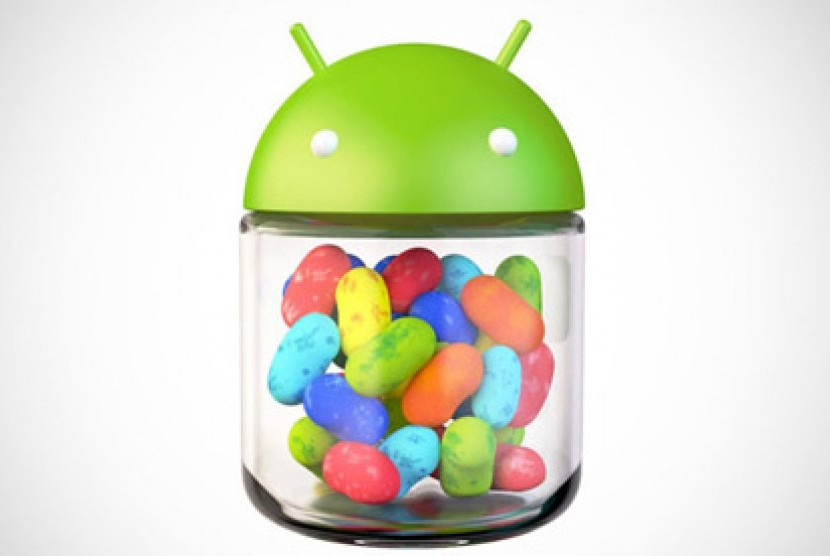
\includegraphics[scale=0.25]{pictures/android-jelly-bean.jpg}
    \caption{Android Jelly Bean}
    \label{}
\end{figure}

Jelly Bean dirilis pada 9 Juli 2012 lewat konferensi I/O Google. Versi ini adalah salah satu versi Android yang kerap mendapatkan update fitur-fitur yang bermanfaat dan menarik, beberapa contohnya semacam memperbaiki rotasi layar, seperti Support resolusi video 4K, Support penulisan huruf Hebrew dan Arabic dari kanan ke kiri, peningkatan kinerja, dan sistem keamanan serta masih banyak lainnya. Fitur yang terdapat pada versi ini adalah : 
\begin{enumerate}
    \item Antarmuka pengguna yang lebih halus:
    \item Waktu vsync pada animasi UI dikelola oleh kerangka kerja Android, termasuk reaksi aplikasi, efek sentuh, komposisi layar, dan penyegaran tampilan
    \item Triple buffering pada grafis
    \item Peningkatan aksesbilitas
    \item Teks dua bahasa dan dukungan bahasa lainnya
    \item Papan ketik yang bisa dimodifikasi oleh pengguna
    \item Perluasan notifikasi
    \item Kemampuan untuk mematikan notifikasi pada aplikasi tertentu
    \item Shortcut dan widget secara otomatis bisa disusun ulang atau diatur ukurannya
    \item Transfer data Bluetooth bagi Android Beam
    \item Diktasi suara luring
    \item Tablet dengan layar kecil bisa menyesuaikan tata letak antarmuka dan layar depan seperti pada telepon pintar
    \item Peningkatan pencarian suara
    \item Peningkatan aplikasi kamera
    \item Google Wallet (pada Nexus 7)
    \item Foto kontak Google+ resolusi tinggi
    \item Aplikasi pencarian Google Now
    \item Audio multi-saluran
    \item Audio USB (bagi suara eksternal DACs)
    \item Audio chaining
    \item Penjelajah web bawaan Android diganti dengan Google Chrome pada perangkat Android pra-instal
    \item Kemampuan untuk menambahkan widget aplikasi tanpa akses root
\end{enumerate}

\item Android 4.4 \textbf{Kitkat}\\
\begin{figure}[!htbp]
    \centering
    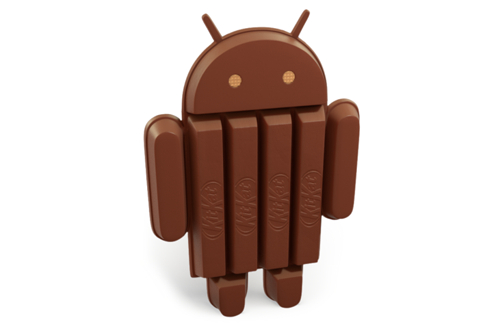
\includegraphics[scale=0.3]{pictures/android-kitkat.jpg}
    \caption{Android Kitkat}
    \label{}
\end{figure}

Android versi inilah yang saat ini banyak dipakai oleh mayoritas masyarakat Indonesia. Kitkat dirilis pada tahun 2013 lalu. pada versi ini, Android banyak mendapatkan pembaharuan/update fitur. Seperti, terdapatnya fitur Screen recording, untuk merekam kegiatan yang terjadi pada layar smartphone, Peningkatan akses notifikasi, New Translucent system UI, System wide settings untuk closed captioning, dan Peningkatan kinerja serta lain sebagainya. Fitur yang terdapat pada versi ini adalah : 
\begin{enumerate}
    \item Pembaruan antarmuka dengan bar status dan navigasi transparan pada layar depan.
    \item Optimasi kinerja pada perangkat dengan spesifikasi yang lebih rendah
    \item Kerangka kerja pencetakan
    \item NFC Host Card Emulation sebagai emulator kartu pintar
    \item WebViews berbasis Chromium
    \item Perluasan fungsionalitas bagi layanan pendengar notifikasi
    \item API umum untuk mengembangkan dan mengelola klien pesan teks, kemampuan untuk menentukan aplikasi SMS standar.
    \item Kerangka kerja baru untuk transisi UI
    \item Kerangka kerja akses penyimpanan untuk mengambil konten dan dokumen dari sumber lain
    \item Sensor batching, Step Detector, dan Counter API
    \item Peningkatan tampilan mode layar penuh, tombol perangkat lunak dan status bar bisa diakses dari tepi dengan cara menggesek
    \item Penyeimbang audio, pemantauan audio, dan peningkatan suara audio
    \item Perekam aktivitas layar yang terintegrasi
    \item Inframerah
    \item Peningkatan aksesibilitas API
    \item Mesin virtual eksperimental baru, ART
    \item Dukungan Bluetooth Message Access Profile (MAP)
\end{enumerate}

\item Android 5.0 \textbf{Lollipop}\\
\begin{figure}[!htbp]
    \centering
    
\includegraphics[scale =0.5]{pictures/android-lolipop.png}
    \caption{Android Lollipop}
    \label{}
\end{figure}

Dirilis pada tahun 2014, Android Lollipop lebih banyak menawarkan fitur tambahan untuk menyempurnakan berbagai fitur yang sudah ada. Dan Nexus 6 merupakan salah satu ponsel yang pertama mencicipi Android Lollipon ini. Selain itu, Google juga lebih menyempurnakan pada kinerja dari Android Lollipop sendiri. Fitur yang terdapat pada versi ini adalah : 
\begin{enumerate}
    \item Desain antarmuka (tampilan) yang dinamakan “Material Design”.
    \item 64-bit ART compiler
    \item Project volta, yang berguna untuk meningkatkan daya hidup baterai 30 persen lebih tahan lama.
    \item ‘factory reset protection’. Fitur ini berguna ketika smartphone hilang, ia tidak bisa direset ulang tanpa memasukkan id google dan kata sandi (password).
\end{enumerate}

\item Android 6.0 \textbf{Marshmallow}\\
\begin{figure}[!htbp]
    \centering
    
\includegraphics[scale=0.3]{pictures/android-marshmallow.jpg}
    \caption{Android Marshmallow}
    \label{}
\end{figure}

Android versi 6.0 dirilis pada tahun 2015 silam, yang banyak membawa pembaharuan. Salah satunya yaitu suda support USB Type-C. Selain itu, Android Marshmallow ini juga terdapat fasilitas autentikasi sidik jari dan daya baterai yang lebih baik. 

Android Marshmallow memperkenalkan model izin yang didesain ulang: sekarang ada hanya delapan kategori izin, dan aplikasi yang tidak lagi secara otomatis diberikan semua hak akses mereka ditentukan pada waktu instalasi. Sebuah sistem opt-in sekarang digunakan, di mana pengguna akan diminta untuk memberikan atau menolak izin individu (seperti kemampuan untuk mengakses kamera atau mikrofon) untuk aplikasi ketika mereka dibutuhkan. Aplikasi mengingat hibah izin mereka, dan mereka dapat disesuaikan oleh pengguna setiap saat. Model izin baru akan digunakan hanya oleh aplikasi yang dikompilasi untuk Marshmallow menggunakan kit pengembangan perangkat lunak (SDK) tersebut, sementara semua aplikasi lainnya akan terus menggunakan model izin sebelumnya.\\

Marshmallow juga memiliki skema manajemen daya baru bernama Doze yang mengurangi tingkat aktivitas aplikasi latar belakang saat perangkat menentukan bahwa itu tidak sedang aktif ditangani oleh pengguna, yang, menurut Google, menggandakan pemakaian baterai perangkat. Hal ini juga memperkenalkan pilihan untuk mengatur ulang semua pengaturan jaringan, tersedia untuk pertama kalinya pada Android, yang membersihkan pengaturan terkait jaringan untuk WI-FI, Bluetooth dan koneksi seluler.

Android Marshmallow memberikan dukungan asli untuk pengenalan sidik jari, memungkinkan penggunaan sidik jari untuk membuka perangkat dan otentikasi Play Store dan pembelian Android Pay; API standar juga tersedia untuk melaksanakan otentikasi berbasis sidik jari dalam aplikasi lain. Android Marshmallow mendukung USB Type-C, termasuk kemampuan untuk menginstruksikan perangkat untuk mengisi daya perangkat lain melalui USB. Marshmallow juga memperkenalkan “pranala yang diverifikasi” yang dapat dikonfigurasi untuk membuka langsung dalam aplikasi tertentu mereka tanpa petunjuk pengguna lanjut.

Versi API Android yang disediakan oleh Marshmallow adalah 23. Alat pengembang Android Marshmallow tersedia di Pengelola SDK di bawah tingkat API “MNC”.

\item Android 7.0 \textbf{Nougat}\\
\begin{figure}[!htbp]
    \centering
    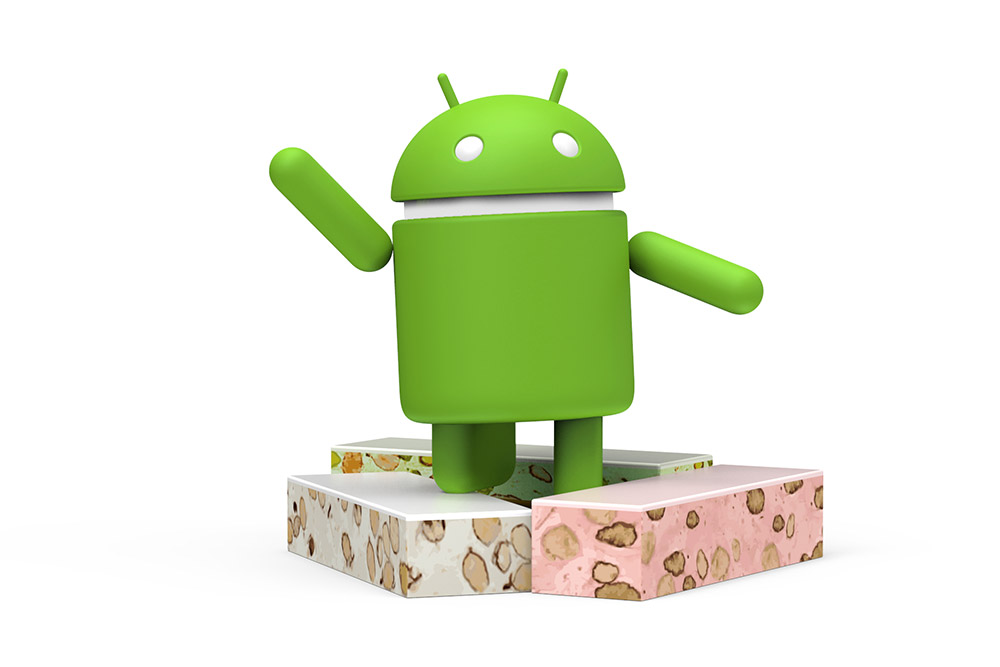
\includegraphics[scale=0.3]{pictures/android-nougat.jpg}
    \caption{Android Nougat}
    \label{}
\end{figure}

Android Nougat versi 7.0 dirilis pada bulan Agustus 2016 yang lebih meningkatkan pada kinerja versi sebelumnya. Selain itu, Android Nougat juga menambah banyak fitur-fitur baru yang diantaranya seperti sudah dapat multitasking, meningkatkan fitur Doze yang dahulu telah dirilis di versi sebelumnya. Inilah beberapa fitur terbaru yang terdapat pada versi Nougat :
\begin{enumerate}
    \item Support Multi window
    \item Dapat langsung membalas pesan dari menu notifikasi atau jendela.
    \item Tampilan panel notifikasi serta quick settings yang baru.
    \item Mode Doze yang lebih baik, (Doze Mode 2.0)
    \item Menu di antara system settings.
\end{enumerate}

\item Android 8.0 \textbf{Oreo}
\begin{figure}[!htbp]
    \centering
    
\includegraphics[scale=0.3]{pictures/android-oreo.jpg}
    \caption{Android Oreo}
    \label{}
\end{figure}

Android versi Oreo dirilis pada bulan Agustus 2017 lalu. Tentu saja Android Oreo merupakan versi final untuk sekarang ini. Beberapa fiturnya juga turut diluncurkan Google selaku pihak pengelola. Adapun fitur-fiturnya tersebut antara lain yaitu :
\begin{enumerate}
    \item Android O lebih berfokus pada kecepatan dan efisiensi
    \item Kecepatan Boot up 2X lebih cepat
    \item Mode Picture in picture lebih flexibel
    \item Aplikasi yang berjalan di latarbelakang atau background lebih diperketat untuk lebih menghemat battery
    \item Battery lebih tahan lama
    \item Emoji yang diperbaharui dan diperbanyak
\end{enumerate}
\end{enumerate}


\chapter{Android Studio}
\begin{figure}[!htbp]
    \centering
    
\includegraphics[scale=0.1]{pictures/android-studio.png}
    \caption{Android Studio}
    \label{}
\end{figure}
Pertama kali muncul Android Inc merupakan sebuah perusahaan software kecil yang didirikan pada bulan Oktober 2003 di Palo Alto, California, USA. Perusahaan ini dibangun oleh beberapa senior di beberpa perusahaan yang berbasis IT dan Communication, Andy Rubin, Rich Miner, Nick Sears dan Chris White. Rubin menyatakan bahwa, Android Inc Didirikan untuk mewujudkan mobile device yang lebih fleksibel terhadap lokasi dan preferensi pemilik. Sehingga, Android Inc ingin mewujudkan mobile device yang lebih mengerti pemiliknya selain karena OS nya yang open source. Berawal dari konsepan inilah Android Inc ternyata menarik minat Google untuk memilikinya. Maka, pada bulan Agustus 2005, Akhirnya Android Inc diakuisisi oleh Google Inc. dan seluruh sahamnya dibeli oleh Google.

Perusahaan milik Andy Rubin, Rich Miner, Nick Sears dan Chris White tetap di Android Inc yang dibeli Google, sehingga akhirnya mereka pun ikut  menjadi bagian dari raksasa Google dan sejarah Android. Disini mereka mulai menggunakan platform Linux untuk membuat sistem operasi bagi mobile phone.Dari sinilah akhirnya banyak pengembang sistem maupun software yang mengembangkan maupun merancang sistem Android menggunakan software – software yang support dengan Android, Contohnya ialah : Android Studio.

Berikut akan diulas beberapa alasan mengapa memahami Android Studio itu penting untuk dilakukan :
\begin{enumerate}
    \item Dengan mempelajari Android Studio dapat membantu Anda untuk mempercepat pembuatan aplikasi yang Anda inginkan.
    \item Android Studio merupakan sebuah tools yang mudah dipahami dan digunakan.
    \item Dalam satu tools ini Anda bisa mendapatkan berbagai manfaat mulai dari pembuatan aplikasi hingga testing aplikasi.
    \item Belajar Android Studio maka Anda bisa menghemat waktu kerja untuk dapat lebih produktif.
    \item Dapat memperdalam ilmu codingan dengan baik. Karena dalam android studi diberikan beberapa referensi ketika Anda mengetik sintaks. Dengan begitu tentunya Anda akan mencari tahu apa saja kegunaan dari sintaks yang terdapat.
    \item Sarana pembelajaran coding dan pembuatan aplikasi yang baik dan praktis hanya dengan Android Studio.
\end{enumerate}

\section{Android Studio}
Pertama kali Android Studio diumumkan di Google I/O Conference pada tahun 2013 dan dirilis ke publik pada tahun 2014. Sebelum lahirnya Android Studio, aplikasi pada Android dikembangkan dengann Eclipse IDE yaitu IDE Java. Setelah adanya android studio yang open source dapat memudahkan bagi Anda yang ingin membuat aplikasi dengan Android Studio.

Android dapat menyediakan interface untuk Anda dalam membuat aplikasi serta mengelola manajemen filen aplikasi anda.  Untuk bahasa programman anda gunakan adalah Java. Dalam Android Studio, anda hanya tinggal menulis, mengedit, menyimpan  dan testing project beserta dan file lainnya yang ada dalam project itu hanya dengan android studio.

Tidak hanya itu, keunggulan menggunakan Android Studio juga memberi Anda akses ke Android Software Development Kit (SDK). SDK adalah sebuah ekstensi dari kode Java yang memperbolehkannya untuk berjalan dengan mulus di device Android. Untuk, Java nya dibutuhkan untuk menulis program, Android SDK sangat diperlukan untuk menjalankan programnya di Android. Maka dari itu dengan menggabungkan keduanya, Anda memerlukan Android Studio. Sehingga ketika Anda menemukan bug pada aplikasi Anda, Anda bisa mengetahui bug tersebut dengan menggunakan Android Studio untuk memperbaikinya.

Berikut ini adalah beberapa fitur Android Studio:
\begin{enumerate}
    \item Environment yang mempermudah Anda untuk mengembangkan aplikasi untuk Android
    \item Support dalam mengembangkan aplikasi Android TV dan Android Wear
    \item Template untuk menentukan design dan komponen Android
    \item Editor layout dengan interface drag-and-drop
    \item Refactoring dan perbaikan cepat khusus Android
    \item Dukungan build berbasis Gradle
    \item Integrasi ProGuard
    \item Emulator yang cepat dan berbagai fitur didalamnya
    \item Dapat terintegrasi dengan Google Cloud Messaging dan App Engine
    \item Dukungan program basic C++ dan NDK
\end{enumerate}

Android Studio adalah Lingkungan Pengembangan Terpadu (Integrated Development Environment/IDE) resmi untuk pengembangan aplikasi Android, yang didasarkan pada IntelliJ IDEA. Selain sebagai editor kode dan fitur developer IntelliJ yang andal, Android Studio menawarkan banyak fitur yang meningkatkan produktivitas Anda dalam membuat aplikasi Android, seperti:
\begin{enumerate}
    \item Sistem build berbasis Gradle yang fleksibel
    \item Emulator yang cepat dan kaya fitur
    \item Lingkungan terpadu tempat Anda bisa mengembangkan aplikasi untuk semua perangkat Android
    \item Terapkan Perubahan untuk melakukan push pada perubahan kode dan resource ke aplikasi yang sedang berjalan tanpa memulai ulang aplikasi
    \item Template kode dan integrasi GitHub untuk membantu Anda membuat fitur aplikasi umum dan mengimpor kode sampel
    \item Framework dan fitur pengujian yang lengkap
    \item Fitur lint untuk merekam performa, kegunaan, kompatibilitas versi, dan masalah lainnya
    \item Dukungan C++ dan NDK
    \item Dukungan bawaan untuk Google Cloud Platform, yang memudahkan integrasi Google Cloud Messaging dan App Engine
\end{enumerate}

Setiap project di Android Studio berisi satu atau beberapa modul dengan file kode sumber dan file resource. Jenis modul meliputi:
\begin{enumerate} 
   \item Modul aplikasi Android
    \item Modul library
    \item Modul Google App Engine
\end{enumerate}

Secara default, Android Studio menampilkan file project Anda dalam tampilan project Android, seperti yang ditunjukkan. Tampilan ini disusun menurut modul untuk memberikan akses cepat ke file sumber utama project Anda. Semua file build terlihat di tingkat teratas di bagian \textbf{Gradle Script} dan setiap modul aplikasi berisi folder berikut:
\begin{enumerate}
    \item manifests: Berisi file AndroidManifest.xml.
    \item java: Berisi file kode sumber Java, termasuk kode pengujian JUnit.
    \item res: Berisi semua resource non-kode, seperti tata letak XML, string UI, dan gambar bitmap.
\end{enumerate}

Struktur project Android pada disk berbeda dengan representasi tersatukan ini. Untuk melihat struktur file project sebenarnya, pilih \textbf{Project} dari menu drop-down Project.

Anda juga dapat menyesuaikan tampilan file project untuk berfokus pada aspek spesifik dari pengembangan aplikasi Anda. Misalnya, memilih tampilan \textbf{Problems} pada project Anda akan menampilkan link ke file sumber yang berisi error coding dan sintaks yang dikenali, seperti tag penutup elemen XML yang tidak ada dalam file tata letak.

\subsection{Langkah Download Android Studio}
Cara mendownload Android studio cukup mudah yaitu dengan \textbf{https://developer.android.com/studio/?gclid=Cj0KEQiAm-CyBRDx65nBhcmVtbIBEiQA7zm8lWCaBd9n9KYYunFXxXsQCPojBVHk5eIH4p9CWM1eLfUaAmd28P8HAQ} yang merupakan laman website resmi Android dan terdapat SDK berbagai macam jenis didalamnya. Tetapi untuk menjalankan Android Studio Anda juga perlu mendownload Java Development Kit dengan \textbf{https://www.oracle.com/technetwork/java/javase/downloads/jdk8-downloads-2133151.html}.

Berikut ini adalah syarat instalasi untuk berbagai sistem operasi :
Windows OS
\begin{enumerate}
    \item Microsoft Windows 7/8/10
    \item Minimum RAM 2GB, direkomendasikan Anda menggunakan RAM 8GB
    \item Minimum space disk tersedia 2GB, tetapi Anda direkomendasikan menyediakan 4GB (500MB untuk IDE, 1,5GB untuk Android SDK, dan emulator sistem gambar)
    \item Resolusi minimum 1280  800
    \item Java Development Kit 8
\end{enumerate}

MAC OS
\begin{enumerate}
    \item MAC OS X 10.8.5 atau lebih – sampai dengan 10.11.4 (El Capitan)
    \item Minimum RAM 2GB, direkomendasikan Anda menggunakan RAM 8GB
    \item Minimum space disk tersedia 2GB, tetapi Anda direkomendasikan menyediakan 4GB (500MB untuk IDE, 1,5GB untuk Android SDK, dan emulator sistem gambar)
    \item Resolusi minimum 1280  800
    \item Java Development Kit 6
 \end{enumerate}

LINUX OS
\begin{enumerate}
    \item Desktop GNOME atau KDE
    \item 64-bit distribution yang bisa menjalankan aplikasi 32-bit
    \item GNU C Library (glibc) 2.11 atau versi selanjutnya
    \item Minimum RAM 2GB
    \item Minimum space disk tersedia 2GB, tetapi Anda direkomendasikan menyediakan 4GB
    \item Resolusi minimum 1280  800
    \item Java Development Kit 8
\end{enumerate}


\subsection{Cara Install Android Studio}
Pertama sebelum anda menginstall Android Studio, Anda harus terlebih dahulu menginstal Java Development Kit-nya. Caranya ialah Anda tinggal membuka installer Java Development Kit yang sudah ada mengunduh sebelumnya, kemudian selanjutnya ikuti langkah yang mereka tunjukkan.

Setelah itu, Anda sudah bisa menginstall Android Studio dengan mengikuti langkah di bawah ini:
\begin{enumerate}
\item Buka installer Android Studio yang sudah ada unduh. Kemudian klik Next.
\item Setelah itu, muncul jendela baru yang memberikan Anda beberapa pilihan komponen apa saja yang ingin Anda install beserta versi android nya. Lalu klik Next.
\item Selanjutnya Anda akan melihat License Agreement, pilih I Agree
\item Setelah itu, Anda akan melihat pilihan lokasi penyimpanan file. Anda tidak perlu mengubah directory yang sudah mereka pilih. Anda tinggal klik Default dan file Anda akan disimpan ke directory yang sudah mereka sediakan. Klik Next dan di layar selanjutnya klik Install.
\item Setelah proses instalasinya selesai klik Next. Kalau sudah, Anda akan melihat windows “Completing Android Studio Setup”. Anda tidak perlu mengubah pilihan Start Android Studio dan langsung saja klik Finish.
\item Setelah itu, Anda akan melihat jendela baru dengan 2 pilihan. Checklist pilihan kedua jika kalian belum pernah menginstall IDE Android Studio sebelumnya dan pilih OK.
\item Setelah itu Anda akan melihat layar WELCOME dari Android Studio dan klik Next.
\item Pilih Standard dan klik Next
\item Anda kemudian akan melihat jendela SDK Component Setup. Pilih komponen yang ingin Anda install dan klik Next. Pada layar selanjutnya klik Finish.
\item Anda kemudian akan melihat layar Downloading Component.
\item Setelah unduhan Anda selesai, proses instalasi Android Studio telah selesai. Anda tinggal klik Finish. Kemudian Anda akan melihat jendela Welcome to Android Studio.
\end{enumerate}

\chapter{Java}
\section{Sejarah Java}
\begin{figure}[!htbp]
    \centering
    
\includegraphics[scale=0.2]{pictures/104-1040733_kotlin-java-programming-language-logo-clipart-1024x598.png}
    \caption{Java}
    \label{}
\end{figure}
Java merupakan bahasa pemrograman yang dapat berjalan pada perangkat komputer maupun telepon genggam.  Bahasa ini dirilis pada tahun 1995 yang  dibuat oleh James Gosling  saat berada di Sun Microsystems  yang  saat ini merupakan bagian dari Oracle. bahasa pemrograman ini mengadopsi penulisan yang terdapat pada C dan C++ yang dikembangkan lagi menjadi sintaksis yang lebih sederhana.  Aplikasi  Dengan basis Java umumnya dikompilasi ke dalam bytecode Dan dapat dijalankan pada mesin virtual Java (JVM). Java  didesain  secara Khusus untuk memanfaatkan implementasi dependensi dengan sangat minimal. Dengan fungsionalitasnya  untuk  berjalan di beberapa platform  sistem operasi yang berbeda sehingga Java memiliki slogan Write once, run anywhere (WORA) atau bisa juga Write once, run everywhere (WORE). Java adalah bahasa pemrograman yang dapat digunakan untuk berbagai macam tujuan.  bahasa pemrograman concurrent, berbasis kelas, dan berorientasi objek. Bahasa ini dirancang secara khusus  untuk mengurangi ketergantungan ketika bahasa ini di terapkan. Hal ini yang dimaksudkan dalam slogannya "Write Once, Run Anywhere (WORA)". Slogan ini memiliki arti bahwa kode yang dijalankan pada suatu platform tidak perlu dikonfirmasi lagi pada platform lainnya. Java merupakan bahasa pemrograman yang paling populer digunakan dan dimanfaatkan dalam pengembangan berbagai jenis perangkat lunak aplikasi ataupun aplikasi lainnya.

Awalnya bahasa pemrograman ini diberi nama Oak, yang Merupakan nama sebuah pohon yang dapat dilihat oleh Gosling dari jendela kantornya. Kemudian dia memberi nama pemrograman ini dengan nama Green,  sehingga akhirnya dia mengganti namanya menjadi Java. Nama ini diambil dari kopi jawa yang banyak dikonsumsi oleh pencipta bahasa pemrograman ini. 

Ketika World Wide Web menjadi populer, Banyak kelebihan yang membuat bahasa ini dapat digunakan dengan baik dan cocok pada proyek maupun alat untuk adaptasi ke web. Pengembang bahasa ini merancang cara agar program berjalan aman pada halaman web dan hingga akhirnya dipilihlah nama yang baru untuk bahasa yaitu Java. Hingga sekarang Java menjadi bahasa pemrograman yang sangat populer digunakan. Aplikasi yang paling populer digunakan adalah aplikasi web client-server dengan 10 juta pengguna.

\section{Sejarah perkembangan}
Pada awalnya pemrograman Java berawal dari The Green Project yang berjalan untuk 18 bulan. Project ini dimulai pada 1991 hingga musim panas 1992. Proyek tersebut belum menggunakan versi Oak .  Proyek ini beranggotakan Patrick Naughton, Mike Sheridan, dan James Gosling, dan sembilan programmer lainnya dari Sun Microsystems.

Proyek ini berlangsung di gedung perkantoran di Sand Hill Road, Menlo Park. Pada saat musim panas 1992 proyek ini ditutup dengan menghasilkan sebuah program Java Oak yang ditujukan sebagai pengendali peralatan dengan teknologi touchscreen seperti sekarang. Teknologi ini diberi nama "*7" (Star Seven).

Setelah era Star Seven, perusahaan TV kabel tertarik untuk menambahkan beberapa orang dari proyek The Green Project. Mereka bekerja pada kantor di 100 Hamilton Avenue, Palo Alto. 

Dengan berjalannya waktu, perusahaan ini semakin maju. Jumlah karyawan yang meningkat dengan sangat signifikan dari 13 orang menjadi 17 orang. Pada saat itu, internet menjadi peran yang menjembatani ide di antara mereka. Pada awal tahun 1990, Internet belum terkenal seperti sekarang sehingga yang dipakai hanyalah untuk akademisi dan militer. Pada maret 1995, source code Java versi 1.0a2 dibuka. 

Ketika itu, pada pukul 04.00 di ruangan hotel Sheraton Pallace terjadi perpecahan di antara anggota proyek The Green Project. Tiga pimpinan proyek itu, Eric Schmidt, George Paolini, dan Masrc Andreessen dari Sun Microsystems membentuk perusahaan Netscape.

\section{Struktur Program}
Struktur program pada bahasa Java dibagi menjadi 4:
\begin{enumerate}
    \item Deklarasi Package\\
    Package merupakan sebuah folder yang diisi dengan  sekumpulan program Java. Deklarasi package biasanya dilakukan saat membuat aplikasi atau membuat program.\\
    Contoh deklarasi package:
    \begin{lstlisting}[language=Java]
package com.proyek.qeuangans;
    \end{lstlisting}
    Pada contoh diatas \textcolor{pred}{com.proyek} merupakan domain dari program proyek. Pada saat membuat program, kita boleh untuk tidak mendeklarasikan package, tetapi saat bagian produksi aplikasi kita wajib menuliskan package.

    \item Import Library\\
    Bagian ini melakukan import library yang dibutuhkan oleh program. Library adalah kumppulan dari class dan fungsi yang bisa kita gunakan ketika membuat program.\\
    Contoh Import Library:
    \begin{lstlisting}[language=Java]
import java.util.Scanner;
    \end{lstlisting}
    Pada contoh diatas, itu berarti kita mengimport class \textcolor{pred}{Scanner} dari sebuah package yang bernama \textcolor{pred}{java.util}

    \item Class\\
    Java merupakan bahasa pemrograman yang berbasis OOP (Object Oriented Programming) yang pada setiap program harus dibungkus di dalam class agar dapat dibuat menjadi objek. Class dibuka dengan kurung buka kurawal \{ dan kurung tutup kurawal \}. Dalam blok class dapat diisi dengan method, fungsi - fungsi dan variable.\\
    Contoh Class:
    \begin{lstlisting}[language=Java]
class NamaProgram {
    public static void main(String args[]){
        System.out.println("Halo Dunia!");
    }
}
    \end{lstlisting}
    Pada contoh program class tersebut terdapat method \textcolor{pred}{main()}. Method main ini akan di eksekusi pertama kali.

    \item Method Main\\
    Method main() merupakan blok program yang pertama kali dieksekusi. Method main() pada java wajib dibuat. Tanpa method main ini, maka program tidak bisa dieksekusi. Method main() memiliki parameter args[]. Parameter ini akan menyimpan sebuah nilai dari sebuah argumen di command line.\\
    Contoh method main:
    \begin{lstlisting}[language=Java]
public static void main(String args[]){
    System.out.println("Halo Dunia!");
}
    \end{lstlisting}

    Fungsi \textcolor{pred}{String args[]} pada baris program diatas adalah sebagai parameter yang berupa array yang memiliki tipe data srting. Parameter - parameter tersebut akan menampung argumen yang akan diberika ke program. 

\end{enumerate}

\subsection{Statement dan Ekspresi pada Java}
Statement dan ekspresi merupakan bagian yang terkecil dalam suatu program. Setiap statement dan ekspresi pada pemrograman java harus diakhiri dengan tanda titik koma (;). Statemen dan ekspresi akan menjadi instruksi yang akan dikerjakan oleh komputer.\\
Contoh Statement dan Ekspresi:
\begin{lstlisting}[language=Java]
System.out.println("Hello World");
System.out.println("Apa kabar?");
var x = 3;
var y = 8;
var z = x + y;
\end{lstlisting}

\subsection{Blok Program Java}
Blok program adalah kumpulan dari beberapa statement dan ekspresi yang dibungkus menjadi satu. Pada blok program ini harus selalu dibuka dengan kurung buka kurawal (\{) dan ditutup dengan kurung tutup kurawal (\}) Blok program dapat juga berisi blok program yang lain atau blok program didalam blok program.
\begin{lstlisting}[language=Java]
// blok program method main
public static void main(String args[]){
    System.out.println("Halo Dunia!");
    System.out.println("Halo para pembaca buku ini");

    // blok program percabangan if
    if( true ){
        System.out.println('True');
    }

    // blok program perulangan for 
    for ( int i = 0; i<10; i++){
        System.out.println("Perulangan ke"+i);
    }
}
\end{lstlisting}

\subsection{Penulisan Komentar pada Java}
Dalam sebuah program, akan ada bagian yang tidak akan pernah di sekssekusi ketika program dijalankan, bagian tersebut adalah komentar.\\
Penulisan komentar pada java sama seperti pada bahasa C. Java dapat mendefinisikan beberapa macam komentar yang diantaranya: 
\begin{itemize}
    \item Single-Line comment\\
    Single-Line comment merupakan penulisan komentar yang digunakan hanya untuk satu baris perintah saja. Biasanya komentar ini menggunakan garis miring ganda \textcolor{pred}{(//)}. Contoh penggunaan Single-Line comment: 
    \begin{lstlisting}[language=Java]
public static void main(String args[]){
    // ini adalah komentar satu baris
}
    \end{lstlisting}

    \item Multiline comment\\
    Multiline comment biasanya digunakan untuk banyak baris perintah atau beberapa baris perintah. Biasanya komentar ini menggunakan garis miring bintang \textcolor{pred}{(/*...*/)}. Contoh penggunaan Multiline comment:
    \begin{lstlisting}[language=Java]
public static void main(String args[]){
    /* awal penggunaan multiline comment
    for ( int i = 0; i<10; i++){
        System.out.println("Perulangan ke"+i);
    }
    akhir penggunaan multiline comment */

}
    \end{lstlisting}

    \item Documentation comment\\
    Documentation ini digunakan untuk menghasilkan file HTML dari program yang kit buat. Biasanya komentar ini dimulai dengan menggunakan tanda \textcolor{pred}{(/** ..... */)}. Contoh penggunaan Documentation comment:
    \begin{lstlisting}[language=Java]
/**
*
*
*
*@author D4TI2B (1184099 dan 1184094)
*@since 2020
*
*
*/
public static void main(String args[]){

}
    \end{lstlisting}

\end{itemize}
Komentar biasanya digunakan untuk beberapa hal:
\begin{enumerate}
    \item Memberi keterangan pada baris kode program
    \item Menonaktifkan fungsi atau method tertentu
    \item Membuat dokumentasi
    \item dll.
\end{enumerate}
%%%%%%%%%%%%%%%%%

\subsection{String dan Character}
String merupakan kumpulan dari Character. Biasanya kita mengetahuinya dengan nama teks. Contoh String:
\begin{lstlisting}[language=Java]
"Hello World"
\end{lstlisting}

Penulisan string pada Java wajib diapit oleh tanda petik ganda seperti pada contoh yang tertulis diatas. Jika diapit dengan tanda petik tunggual, maka dibuat menjadi character. Contoh penggunaan:
\begin{lstlisting}
'Hello world'
\end{lstlisting}

%Jadi harap dibedakan:
%\begin{enumerate}
%    \item Tanda petik ganda ("...") untuk membuat string;
%    \item Sedangkan tanda petik tunggal ('...') untuk membuat karakter.
%\end{enumerate}

\subsection{Case Sensitive}
Java memiliki sifat Case Sensitive, case sensitive disini berarti perbedaan huruf kapital dan huruf kecil harus diperhatikan karena banyak orang yang sering melakukan kesalahan dalam hal ini. Karena masih banyak orang yang belum bisa membedakan mana variabel yang menggunakan huruf besar dan huruf kecil.

\section{Mengenal Tipe Data Dasar di Java}
Tipe data merupakan bagian penting dalam pemrograman java. Tipe data biasanya akan digunakan dalam bentuk variabel variabbel. Java memiliki banyak tipe data dasar atau yang biasa dikenal tipe data primitif pada java. Tipe data dasar atau primitif dibagi menjadi empat bagian:
\begin{enumerate}
    \item Integer\\
    Integer merupakan tipe data untuk data bilangan bulat. Tipe data integer terbagi lagi menjadi empat bagian yaitu:
    \begin{itemize}
        \item byte
        \item short
        \item Int
        \item Long
    \end{itemize}
    Semakin besarnya tipe data maka akan semakin besar pula nilai yang dapat ditampung oleh tipe data tersebut.

    \item Floating Point\\
    Floating point merupakan type data rasional, tipe data ini dibagi menjadi dua bagian yaitu:
    \begin{itemize}
        \item Float
        \item Double 
    \end{itemize}

    \item Char\\
    Char merupakan simbol dari sebuah character. Terdapat kurang lebih 256 simbol yang terdaftar  dalam kode ASCII. 

    \medskip

    \noindent\fcolorbox{red}{yellow}{%
        \minipage[b]{\dimexpr\linewidth\fboxsep\fboxrule\relax}
        ASCII (American Standard Code for Information Interchange) merupakan Kode Standar Amerika untuk Pertukaran Informasi atau sebuah standar internasional dalam pengkodean huruf dan simbol secara universal. \cite{webmateridosen1}
        \endminipage}

    \medskip

    \item Boolean
    Boolean merupakan tipe data yang paling sederhana dalam pemrograman karena tipe data ini hanya memiliki dua jenis saja yaitu:
    \begin{itemize}
        \item True
        \item False
    \end{itemize}
    Nilai dari boolean ini, sering digunakan untuk mengatur alur dari jalannya program. Boolean lebih sering digunakan untuk percabangan pada program.
    \cite{ahmadi1}
    
\end{enumerate}

Berikut ini jangkauan nilai yang dapat diterapkan pada tipe data primitif diatas:
\begin{table}[htbp!]
    \begin{tabular}{|l|l|l|l|}
    \hline
    \rowcolor[HTML]{9AFF99} 
    \textbf{Tipe Data} & \textbf{Besar Storage} & \textbf{Nilai Minimal} & \textbf{Nilai Maksimal} \\ \hline
    Byte               & 8 bit (1 byte)         & -128                   & 127                     \\ \hline
    Short              & 16 bit (2 byte)        & -32768                 & 32767                   \\ \hline
    Int                & 32 bit (4 byte)        & -2147483648            & 2147483647              \\ \hline
    Long               & 64 bit (8 byte)        & -9223372036854775808   & 9223372036854775807     \\ \hline
    Float              & 32 bit (4 byte)        & 3.4 E-38              & 3.4 E+38               \\ \hline
    Double             & 64 bit (8 byte)        & 1.7 E-308             & 1.7 E+308              \\ \hline
    Char               & 16 bit (2 byte)        & \textbackslash{}uoooo  & \textbackslash{}uffff   \\ \hline
    \end{tabular}
    \caption{Jangkauan nilai tipe data primitif}
    \medskip
    \noindent\fcolorbox{red}{yellow}{%
        \minipage[h!]{\dimexpr\linewidth\fboxsep\fboxrule\relax}
        Tipe data tersebut dapat dibuat menjadi array. Tanda array adalah dengan adanya kurung siku "[]" pada saat setelah mengetik tipe data yang digunakan.
        \endminipage}
    \medskip
    \end{table}

\newpage
\section{Variabel}
Variabel adalah tempat untuk menampung sejumlah value pada memori. Jika dianalogikan, Variabel dapat dimisalkan seperti sebuah ruangan. 

Berikut ini adalah beberapa para ilmuan yang memberikan pengertian dari variabel :
\begin{enumerate}
    \item F.N Kerlinger\\
Pengertian variabel menurut F.N Kerlinger merupakan suatu konsep yang memiliki macam-macam nilai dari suatu konsep yang dapat di rubah. Sehingga konsep tersebut akan mendapatkan titik kesimpulan yang tepat dan terbaik. \cite{FNKerlinger}

    \item Sutrisno Hadi\\
Variabel merupakan variasi dari objek penelitian, seperti tinggi badan manusia yang divariasikan dengan berat badan maupun usia yang dimiliki. Sehingga menghasilkan nilai kuantitatif dari suatu penelitian yang diterapkan secara real atau nyata.

    \item Sugiono\\
Pengertian Variabel dari Sugiono merupakan segala sesuatu yang diproses melalui informasi tentang suatu hal dari penelitian untuk dipelajari dan mendapatkan hasil dari penelitian tersebut. Yang mana akan ada kesimpulan dari proses penelitiannya.

    \item Freddy Rankuti\\
Freddy Rankuti menerapkan variabel dengan artian suatu konsep yang memiliki nilai bervariasi. Yang mana nilai tersebut dibagi menjadi 4 data yang berbeda. Seperti rasio, skala, ordinal, nominal dan internal.

    \item Suharsimi Arikunto\\
Variabel merupakan objek penelitian yang menjadi perhatian pada suatu titik objek penelitian. Yang nantinya akan mendapatkan nilai dari kesimpulan suatu proses.

    \item Bagja Waluya\\
Konsep yang tidak pernah ketinggalan dalam setiap eksperimen yang dilakukan oleh seseorang. Dari eksperimen tersebut akan menghasilkan suatu data yang berguna sebagai bukti otentik suatu penelitian.

    \item Moh. Nazir\\
Berikutnya, mengenai pengertiaan variabel menurut Moh. Nazir adalah suatu konsep yang memiliki bermacam-macam nilai yang nyata. Dalam suatu penelitian yang menghasilkan garis besar dari adanya nilai kualitas dan kuantitas.

    \item Sugiarto\\
Menurut Sugiarto variabel adalah suatu karakter yang dapat di observasi dari unit amatan yang merupakan pengenal atau atribut dari anggota kelompok. Maksud dari variabel ini adalah terjadinya proses variasi antara objek satu dengan objek yang lain. Yang mana aturan masing-masing kelompok memiliki perbedaan variasi.

    \item Tri Mutiara\\
Suatu proses yang berjalan dengan baik hingga mendapat perhatian dengan fokus pada pengaruh nilai yang value. Itulah pengertian variabel menurut Tri Mutiara. Yang mengartikan variabel sebagai cara terbaik mendapatkan hasil penelitian.

    \item Bhisma Murti\\
Definisi variabel menurut bhisma murti adalah adanya fenomena yang memiliki variasi nilai pada sebuah observasi. Yang mana variasi nilai itu dapat di kukur dengan cara kualitatif dan kuantitatif. Sehingga menghasilkan data yang benar dan tepat.

    \item Dr Ahmad Watik Pratiknya\\
Konsep yang memiliki variabilitas dengan penggambaran suatu abstraksi dari fenomena tertentu. Yang mana konsep tersebut berupa data seperti asal kepemilikan ciri yang bervariasi, inilah yang disebut variabel.
\end{enumerate}

\textbf{Variabel pada java dibagi menjadi dua yaitu:}
\begin{itemize}
    \item Variabel Lokal\\
    Variabel lokal merupakan variabel yang hanya dapad diakses pada lingkup khusus saja. Variabel ini biasanya hanya bisa diakses pada prosedur atau fingsi dimana prosedur tersebut di deklarasikan. 
    \item Variabel Global\\
    Variabel Global merupakan variabel yang dapat diakses melalui semua lingkup dalam program yang dibuat. Variabel Global ini dapat digunakan oleh semua fungsi dan prosedur.
\end{itemize}

Untuk mendeklarasikan variabel, Kita harus menulis terlebih dahulu tipe data dari variabelnya, kemudian nama variabel, setelah itu kita wajib menginisiasi variabel tersebut agar tidak terjadi error. 

Berikut merupakan standar-standar dalam penulisan variabel:
\begin{enumerate}
\item Nama variabel biasanya diawali dengan huruf atau garis bawah. Contoh:
\begin{lstlisting}[language=Java]
nama = "Nama Kalian";
_nama = "Nama Kalian";
namaKu = "Nama Kalian";
nama_variabel = "Nama Kalian";
\end{lstlisting}

\item Karakter selanjutnya pada variabel dapat berupa huruf, garis bawah maupun angka. Contoh:
\begin{lstlisting}[language=Java]
__nama = "Nama Kalian"
nama1 = "Nama Kalian"
x1 = "Nama Kalian"    
\end{lstlisting}

\item  Nama variabel tidak boleh diawali dengan angka. Contoh:
\begin{lstlisting}[language=Java]
/* Penggunaan variabel ini salah karena diawali dengan angka */
3nama = "Nama Kalian"    
\end{lstlisting}

\item Penulisan variable bersifat Case-Sensitive (huruf besar dan huruf kecil sangant berpengaruh), contoh: 
\begin{lstlisting}[language=Java]
NAMA = "Nama Kalian"
nama = "Nama Kalian"
\end{lstlisting}
Variable nama dan NAMA pada contoh diatas merupakan variabel yang berbeda, dan memiliki arti yang berbeda.

\item Nama variabel yang digunakan tidak boleh menggunakan kata kunci yang ada pada bahasa pemrograman java (Reserved Word), contoh: 
\begin{lstlisting}[language=Java]
/* Penggunaan Variable seperti ini salah karena menggunakan reserved word pada java. */
if = "Nama saya: "
else = "Nama anda:"
while = "Nama kami:"    
\end{lstlisting}
\end{enumerate}


\section{Dasar - dasar Pemrograman}
\subsection{Operator}
Pada setiap pemrograman, operator merupakan peran penting karena tanpa adanya operator maka program tidak akan bisa berjalan dengan sempurna. Pada java, operator dibagi menjadi 6 jenis operator yaitu:
\begin{itemize}
    \item Operator Aritmatika
    \item Operator Penugasan
    \item Operator Logika
    \item Operator Pembanding 
    \item Operator Bitwise
    \item Operator Ternary
\end{itemize}

Dari keenam operator tersebut tentunya akan kami jabarkan satu per satu. 
\begin{enumerate}
    \item \textbf{Operator Aritmatika}\\
    Operator aritmatika digunakan untuk melakukan operasi aritmatika.
    \begin{table}[h!]
        \begin{center}
            \begin{tabular}{|l|l|}
                \hline
                \rowcolor[HTML]{9AFF99} 
                \textbf{Nama}           & \textbf{Simbol} \\ \hline
                Penjumlahan             & +               \\ \hline
                Pengurangan             & -               \\ \hline
                Perkalian               & *               \\ \hline
                Pembagian               & /               \\ \hline
                Sisa bagi (Mod/Modulus) & \%              \\ \hline
                \end{tabular}
        \end{center}      
        \caption{Operator Aritmatika}
    \end{table}

    Contoh penggunaan operator aritmatika pada program:
    \begin{lstlisting}[language=Java]
//Penjumlahan
total = angka1 + angka2;
System.out.println("Total = " + total);

//Pengurangan
total = angka1 - angka2;
System.out.println("Total = " + total);

//Perkalian
total = angka1 * angka2;
System.out.println("Total = " * total);

//Pembagian
total = angka1 / angka2;
System.out.println("Total = " + total);

//Modulus (sisa bagi)
total = angka1 % angka2;
System.out.println("Total = " + total);
    \end{lstlisting}

    \item \textbf{Operator Penugasan}\\
    Operator penugasan atau biasa disebut \textit{Assignment Operator} digunakan untuk memberikan sebuah tugas pada variable tertentu untuk mengisi nilai. Operator penugasan terdiri dari:
    \begin{table}[h!]
        \begin{center}
        \begin{tabular}{|l|l|}
            \hline
            \rowcolor[HTML]{9AFF99} 
            \textbf{Nama}             & \textbf{Simbol} \\ \hline
            Pengisian Nilai           & =               \\ \hline
            Pengisian dan Penambahan  & +=              \\ \hline
            Pengisian dan Pengurangan & -=              \\ \hline
            Pengisian dan Perkalian   & *=              \\ \hline
            Pengisian dan Pembagian   & /=              \\ \hline
            Pengisian dan Sisa bagi   & \%=             \\ \hline
            \end{tabular}
            \caption{Operator Penugasan}
        \end{center}
    \end{table}
    Contoh penggunaan operator penugasan:
    \begin{itemize}
        \item Pengisian Nilai
        \begin{lstlisting}[language=Java]
int x;
int y;

// Pengisian nilai
x = 5;
y = 10;
System.out.println("x : " + x);
System.out.println("y : " + y);
        \end{lstlisting}
        Hasil ketika program dijalankan:
        \begin{figure}[htbp!]
            \centering
            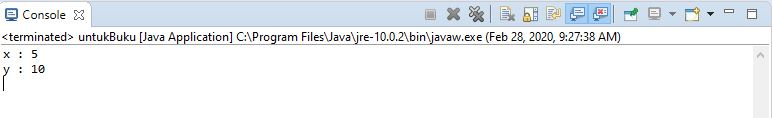
\includegraphics[scale=0.6]{pictures/Pengisian_Nilai_Operator_Penugasan.jpg}
            \caption{Hasil Pengisian Nilai Operator Penugasan}
            \label{}
        \end{figure}

        \item Penambahan
        \begin{lstlisting}[language=Java]
int x;
int y;
x = 5;
y = 10;

// penambahan
y += x;

// Hasil y menjadi 15
System.out.println("Penambahan : " + y);
        \end{lstlisting}
        Hasil ketika program dijalankan:
        \begin{figure}[htbp!]
            \centering
            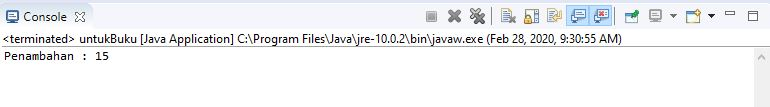
\includegraphics[scale=0.6]{pictures/penambahan_operator_penugasan.JPG}
            \caption{Hasil Penambahan Operator Penugasan}
            \label{}
        \end{figure}

        \item Pengurangan
        \begin{lstlisting}[language=Java]
int x;
int y;
x = 5;
y = 10;

// Pengurangan 
y -= x;

// Hasil y menjadi 5
System.out.println("Pengurangan : " + y);
        \end{lstlisting}
        Hasil ketika program dijalankan:
        \begin{figure}[htbp!]
            \centering
            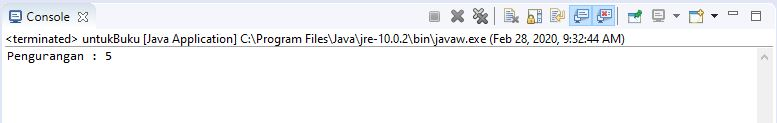
\includegraphics[scale=0.6]{pictures/pengurangan_operator_penugasan.JPG}
            \caption{Hasil Pengurangan Operator Penugasan}
            \label{}
        \end{figure}

        \item Perkalian
        \begin{lstlisting}[language=Java]
int x;
int y;
x = 5;
y = 10;

// Perkalian 
y *= x;

// Hasil y menjadi 50
System.out.println("Perkalian : " + y);
        \end{lstlisting}
        Hasil ketika program dijalankan:
        \begin{figure}[htbp!]
            \centering
            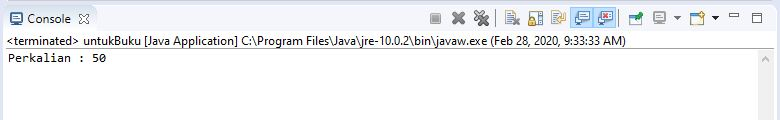
\includegraphics[scale=0.6]{pictures/perkalian_operator_penugasan.JPG}
            \caption{Hasil Perkalian Operator Penugasan}
            \label{}
        \end{figure}
\newline
        \item Pembagian
\begin{lstlisting}[language=Java]
int x;
int y;
x = 5;
y = 10;

// Pembagian 
y /= x;

// Hasil y menjadi 2
System.out.println("Pembagian : " + y);
\end{lstlisting}
\begin{figure}[htbp!]
    \centering
    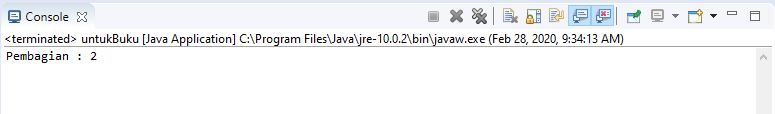
\includegraphics[scale=0.6]{pictures/pembagian_operator_penugasan.JPG}
    \caption{Hasil Pembagian Operator Penugasan}
    \label{}
\end{figure}

        \item Sisa bagi
        \begin{lstlisting}[language=Java]
int x;
int y;
x = 5;
y = 10;

// Pengurangan 
y %= x;

// Hasil y menjadi 0
System.out.println("Sisa Bagi : " + y);
        \end{lstlisting}
        Hasil ketika program dijalankan:
        \begin{figure}[htbp!]
            \centering
            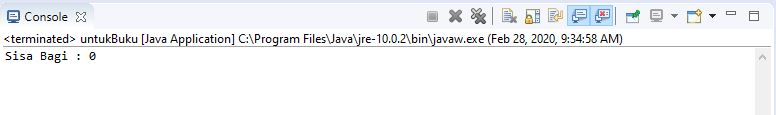
\includegraphics[scale=0.6]{pictures/sisa_bagi_operator_penugasan.JPG}
            \caption{Hasil Sisa Bagi Operator Penugasan}
            \label{}
        \end{figure}
    \end{itemize}

    \newpage
    \item \textbf{Operator Logika}\\
    Operator Logika merupakan operator yang akan sering kalian temui pada saat membuat sebuah program. Operator logika hanya bernilai \textbf{true} atau \textbf{false}. Jenis - jenis operator logika:
    \begin{table}[h!]
        \centering
        \begin{tabular}{|l|l|}
        \hline
        \rowcolor[HTML]{9AFF99} 
        \textbf{Nama}      & \textbf{Simbol} \\ \hline
        Logika AND         & \&\&            \\ \hline
        Logika OR          & ||              \\ \hline
        Negasi / Kebalikan & !               \\ \hline
        \end{tabular}
        \caption{Operator Logika}
    \end{table}

    Contoh penggunaan operator:
    \begin{itemize}
        \item \textbf{Logika AND}
        \begin{lstlisting}[language=Java]
public static void main(String[] args) {
    int a = 5;
    int b = 10;
    //Hasil Perbandingan a dan b benar keduanya maka Hasil = true
    boolean hasil_satu = (a > 1) && (b > 5);
    System.out.println("Hasil Pertama: " + hasil_satu);
    
    //Hasil Perbandingan a dan b hanya benar salah satunya saja maka Hasil = false
    boolean hasil_dua = (a > 1) && (b < 5);
    System.out.println("Hasil Kedua: " + hasil_dua);
}            
        \end{lstlisting}
        Hasil dari program tersebut adalah:
        \begin{figure}[htbp!]
            \centering
            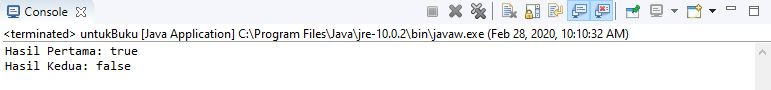
\includegraphics[scale=0.6]{pictures/hasil_operator_logika_AND.JPG}
            \caption{Hasil Operator Logika AND}
            \label{}
        \end{figure}

        \item \textbf{Logika OR}
        \begin{lstlisting}[language=Java]
public static void main(String[] args) {
    int a = 5;
    int b = 10;
                
    //Hasil Perbandingan a dan b hanya benar salah satunya, Tertapi jika menggunakan logika OR meskipun hanya benar salah satu maka akan menghasilkan nilai true
    boolean hasil_satu = (a > 1) || (b < 5);
    System.out.println("Hasil Kedua: " + hasil_satu);
}            
        \end{lstlisting}
        Hasil dari program tersebut adalah:
        \begin{figure}[htbp!]
            \centering
            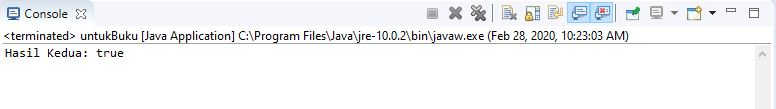
\includegraphics[scale=0.6]{pictures/hasil_operator_logika_OR.JPG}
            \caption{Hasil Operator Logika OR}
            \label{}
        \end{figure}

        \item \textbf{Negasi / Kebalikan}
        \begin{lstlisting}[language=Java]
public static void main(String[] args) {
    int a = 5;
    int b = 10;
                
    boolean hasil_dua = !((a < 15) ^ (b > 6));
    System.out.println("Hasil Kedua: " + hasil_dua);
}
        \end{lstlisting}
        Hasil dari program tersebut adalah:
        \begin{figure}[htbp!]
            \centering
            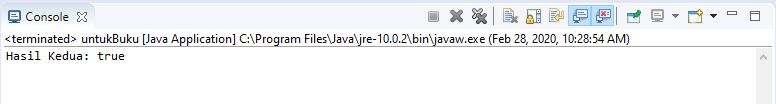
\includegraphics[scale=0.6]{pictures/hasil_operator_logika_negasi.JPG}
            \caption{Hasil negasi/kebalikan}
            \label{}
        \end{figure}

    \end{itemize}
    Pada penggunaan operator logika ini, kita dapat melihat tabel kebenaran untuk mendapatkan hasil dari logika.
    \begin{table}[h!]
        \centering
        \begin{tabular}{|l|l|c|c|}
            \hline
            \rowcolor[HTML]{9AFF99} 
            \textbf{Pernyataan 1}        & \textbf{Pernyataan 2}        & \multicolumn{1}{l|}{\cellcolor[HTML]{9AFF99}\textbf{AND}} & \multicolumn{1}{l|}{\cellcolor[HTML]{9AFF99}\textbf{OR}} \\ \hline
            {\color[HTML]{3166FF} true}  & {\color[HTML]{3166FF} true}  & {\color[HTML]{3166FF} true}                               & {\color[HTML]{3166FF} true}                              \\ \hline
            {\color[HTML]{3166FF} true}  & {\color[HTML]{FE0000} false} & {\color[HTML]{FE0000} false}                              & {\color[HTML]{3166FF} true}                              \\ \hline
            {\color[HTML]{FE0000} false} & {\color[HTML]{3166FF} true}  & {\color[HTML]{FE0000} false}                              & {\color[HTML]{3166FF} true}                              \\ \hline
            {\color[HTML]{FE0000} false} & {\color[HTML]{FE0000} false} & {\color[HTML]{FE0000} false}                              & {\color[HTML]{FE0000} false}                             \\ \hline
            \end{tabular}
        \caption{Tabel Kebenaran}
        \end{table}


\newpage
    \item \textbf{Operator Perbandingan}\\
    Operator perbandingan fungsinya adalah membandingkan. Operator ini akan menghasilkan nilai berupa boolean. Boolean berarti hasil ini hanya berupa \textbf{true} atau \textbf{false}. Jenis - jenis operator logika:
    \begin{table}[h!]
        \centering
        \begin{tabular}{|l|c|}
        \hline
        \rowcolor[HTML]{9AFF99} 
        \textbf{Nama}           & \multicolumn{1}{l|}{\cellcolor[HTML]{9AFF99}\textbf{Simbol}} \\ \hline
        Lebih Besar             & \textgreater{}                                               \\ \hline
        Lebih Kecil             & \textless{}                                                  \\ \hline
        Sama Dengan             & ==                                                           \\ \hline
        Tidak Sama Dengan       & !=                                                           \\ \hline
        Lebih Besar Sama Dengan & \textgreater{}=                                              \\ \hline
        Lebih Kecil Sama Dengan & \textless{}=                                                 \\ \hline
        \end{tabular}
        \caption{Operator Perbandingan}
        \end{table}

        Contoh penggunaan operator:
        \begin{itemize}
            \item \textbf{Lebih Besar}
            \begin{lstlisting}[language=Java]
public static void main(String[] args) {
    int A = 12;
    int B = 4;
    boolean hasil;
            
    // Apakah nilai A lebih besar dari nilai B?
    hasil = A > B;
    System.out.println(hasil);
}                
            \end{lstlisting}
            Hasil Eksekusi Program:
            \begin{figure}[htbp!]
                \centering
                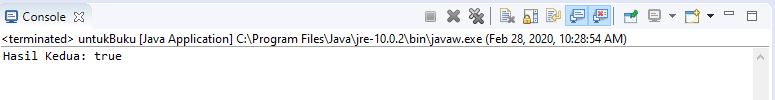
\includegraphics[scale=0.6]{pictures/operator_perbandingan_lebih_besar.JPG}
                \caption{Hasil operator lebih besar}
                \label{}
            \end{figure}
            \newpage
            \item \textbf{Lebih Kecil}
            \begin{lstlisting}[language=Java]
public static void main(String[] args) {
    int A = 12;
    int B = 4;
    boolean hasil;

    // Apakah nilai A lebih kecil dari nilai B?
    hasil = A < B;
    System.out.println(hasil);
}
            \end{lstlisting}
            Hasil Eksekusi Program:
            \begin{figure}[htbp!]
                \centering
                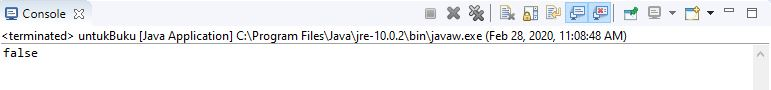
\includegraphics[scale=0.6]{pictures/operator_perbandingan_lebih_kecil.JPG}
                \caption{Hasil operator lebih kecil}
                \label{}
            \end{figure}

            \item \textbf{Sama Dengan}
            \begin{lstlisting}[language=Java]
public static void main(String[] args) {
    int A = 12;
    int B = 4;
    boolean hasil;

    // Apakah nilai A sama dengan nilai B?
    hasil = A == B;
    System.out.println(hasil);
}
            \end{lstlisting}
            Hasil Eksekusi Program:
            \begin{figure}[htbp!]
                \centering
                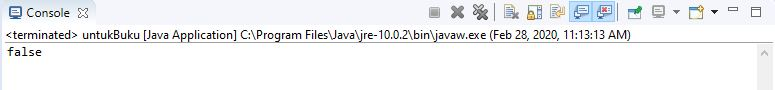
\includegraphics[scale=0.6]{pictures/operator_perbandingan_sama_dengan.JPG}
                \caption{Hasil operator sama dengan}
                \label{}
            \end{figure}

            \item \textbf{Tidak Sama Dengan}
            \begin{lstlisting}[language=Java]
public static void main(String[] args) {
    int A = 12;
    int B = 4;
    boolean hasil;
            
    // Apakah nilai A tidak sama dengan nilai B?
    hasil = A != B;
    System.out.println(hasil);
}
            \end{lstlisting}
            Hasil Eksekusi Program:
            \begin{figure}[htbp!]
                \centering
                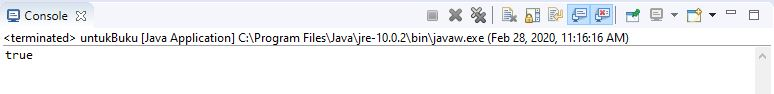
\includegraphics[scale=0.6]{pictures/operator_perbandingan_tidak_sama_dengan.JPG}
                \caption{Hasil operator tidak sama dengan}
                \label{}
            \end{figure}

            \item \textbf{Lebih Besar Sama Dengan}
            \begin{lstlisting}[language=Java]
public static void main(String[] args) {
    int A = 12;
    int B = 4;
    boolean hasil;
            
    // Apakah nilai A lebih besar atau sama dengan nilai B?
    hasil = A >= B;
    System.out.println(hasil);
}
            \end{lstlisting}
            \begin{figure}[htbp!]
                \centering
                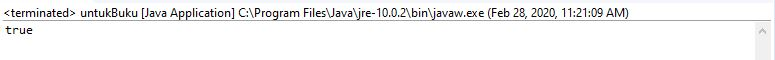
\includegraphics[scale=0.6]{pictures/operator_perbandingan_lebih_besar_sama_dengan.JPG}
                \caption{Hasil operator lebih besar sama dengan}
                \label{}
            \end{figure}

            \item \textbf{Lebih Kecil Sama Dengan}
            \begin{lstlisting}[language=Java]
public static void main(String[] args) {
    int A = 12;
    int B = 4;
    boolean hasil;
            
    // Apakah nilai A lebih kecil atau sama dengan nilai B?
    hasil = A <= B;
    System.out.println(hasil);
}
            \end{lstlisting}
            Hasil Eksekusi Program:
            \begin{figure}[htbp!]
                \centering
                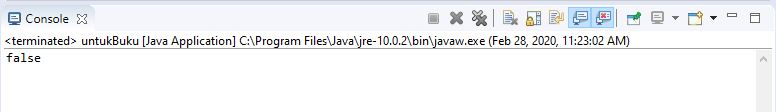
\includegraphics[scale=0.6]{pictures/operator_perbandingan_lebih_kecil_sama_dengan.JPG}
                \caption{Hasil operator lebih kecil sama dengan}
                \label{}
            \end{figure}

        \end{itemize}


    \item \textbf{Operator Bitwise}\\
    Operator bitwise fungsinya hampir sama dengan operator logika. Namun perbedaannya adalah operator bitwise digunakan untuk bilangan biner saja (bit). Operator bitwise terdir dari:
    \begin{table}[h!]
        \centering
        \begin{tabular}{|l|c|}
        \hline
        \rowcolor[HTML]{9AFF99} 
        \textbf{Nama}          & \multicolumn{1}{l|}{\cellcolor[HTML]{9AFF99}\textbf{Simbol}} \\ \hline
        AND                    & \&                                                           \\ \hline
        OR                     & |                                                            \\ \hline
        XOR                    & \textasciicircum{}                                           \\ \hline
        Negasi / Kebalikan     & $\sim$                                                       \\ \hline
        Left Shift             & \textless{}\textless{}                                       \\ \hline
        Right Shift            & \textgreater{}\textgreater{}                                 \\ \hline
        Left Shift (Unsigned)  & \textless{}\textless{}\textless{}                            \\ \hline
        Right Shift (Unsigned) & \textgreater{}\textgreater{}\textgreater{}                   \\ \hline
        \end{tabular}
        \caption{Operator Bitwise}
    \end{table}
    \newline
    Contoh penggunaan aplikasi bitwise:
    \begin{lstlisting}[language=Java]
        public static void main(String[] args) {
        int a = 60;    /* 60 = 0011 1100 */
        int b = 13;    /* 13 = 0000 1101 */
        int c = 0;

        c = a & b;       /* 12 = 0000 1100 */
        System.out.println("a & b = " + c);

        c = a | b;       /* 61 = 0011 1101 */
        System.out.println("a | b = " + c);

        c = a ^ b;       /* 49 = 0011 0001 */
        System.out.println("a ^ b = " + c);

        c = ~a;          /*-61 = 1100 0011 */
        System.out.println("~a = " + c);

        c = a << 2;     /* 240 = 1111 0000 */
        System.out.println("a << 2 = " + c);

        c = a >> 2;     /* 215 = 1111 */
        System.out.println("a >> 2  = " + c);

        c = a >>> 2;     /* 215 = 0000 1111 */
        System.out.println("a >>> 2 = " + c);
    }        
    \end{lstlisting}
    Hasil yang dikeluarkan adalah:
    \begin{figure}[htbp!]
        \centering
        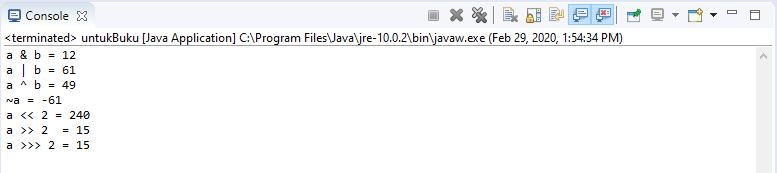
\includegraphics[scale=0.6]{pictures/operator_bitwise.JPG}
        \caption{Hasil Operator Bitwise}
        \label{}
    \end{figure}
\end{enumerate}

\section{Percabangan pada Java}
Percabangan merupakan pemilihan keputusan untuk mengeksekusi program berdasarkan kondisi yang ditetapkan. \cite{HengkyPercabangan}

Percabangan biasa disebut juga dengan \textit{Control Flow} yang merupakan perintah pada program agar program dapat mengambil keputusan. Percabangan akan menggunakan nilai \textbf{true} atau \textbf{false} dari beberapa kondisi yang terjadi.\\

Pada dasarnya dalam pemrograman terdapat 3 macam percabangan:
\begin{enumerate}
    \item Percabangan IF
    \item Percabangan IF/ELSE 
    \item Percabangan IF/ELSE/IF 
    \item Percabangan CASE
\end{enumerate}

\newpage
\subsection{Percabangan IF}
\begin{figure}[h!]
    \centering
    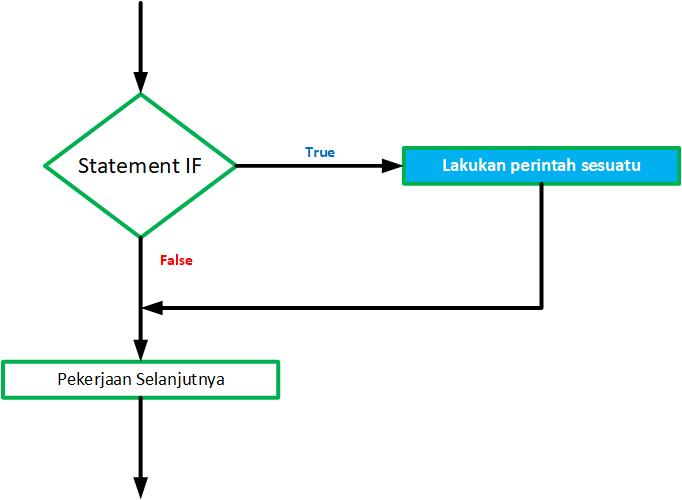
\includegraphics[scale=0.4]{pictures/flowmap_if.jpg}
    \caption{Alur logika percabangan IF}
    \label{}
\end{figure}
Percabangan IF hanya punya satu pilihan dan hanya akan dikerjakan kalau \textit{statementnya} bernilai benar. Jika \textit{statement} tidak bernilai benar, maka percabangan ini tidak bisa dijalankan. Bentuk dari IF adalah:
\begin{lstlisting}[language=Java]
if( statement ) {
    // perintah jika statement bernilai benar
    // perintah 1
    // perintah 2
    // dan seterusnya
}    
\end{lstlisting}

\textbf{Statement} hanya akan menghasilkan nilai \textbf{True} atau \textbf{False}. Untuk pengisian statement dapat digabungkan dengan operator logika, perbandingan, dan berbagai operator yang dapat digunakan dalam program. 

\medskip

\noindent\fcolorbox{red}{yellow}{%
    \minipage[b]{\dimexpr\linewidth\fboxsep\fboxrule\relax}
    Contoh dalam kegiatan sehari - hari adalah ketika kita belanja. Misalkan kita berbelanja diatas nominal 200.000 maka akan mendapat potongan harga.
    \endminipage}

\medskip

Jika contoh tersebut dibuat menjadi program maka akan menjadi:
\begin{lstlisting}[language=Java]
public static void main(String[] args) {

    // membuat variabel belanja dan scanner
    int belanja = 0;
    Scanner scan = new Scanner(System.in);

    // mengambil input
    System.out.print("Total Belanjaan: Rp ");
    belanja = scan.nextInt();

    // cek apakah dia belanja di atas 100000
    if ( belanja > 100000 ) {
        System.out.println("Selamat, anda mendapatkan hadiah!");
    }

    System.out.println("Terima kasih...");
}

\end{lstlisting}

\subsection{Percabangan IF/ELSE}
\begin{figure}[h!]
    \centering
    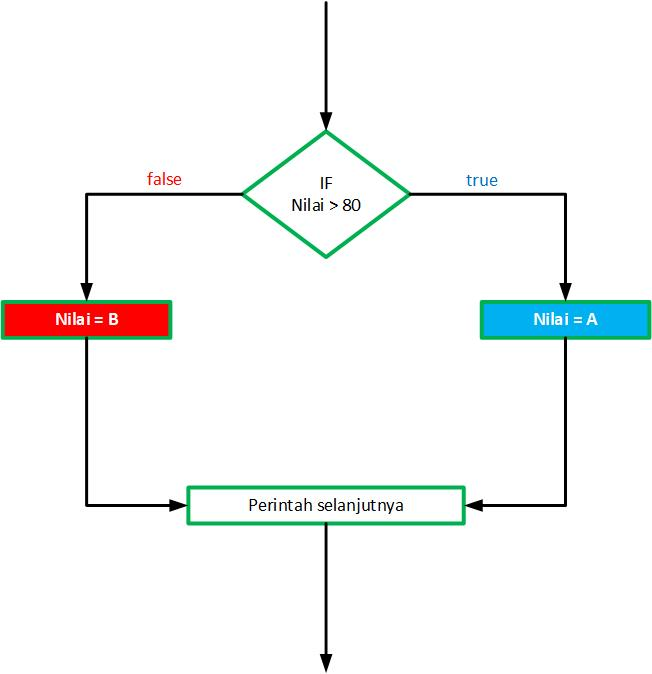
\includegraphics[scale=0.4]{pictures/flowmap_if_else.jpg}
    \caption{Alur logika percabangan if else}
    \label{}
\end{figure}

Percabangan IF/ELSE pada dasarnya hampir sama dengan percabangan IF diatas. Namun IF/ELSE memiliki perintah alternatif jika statement yang dijalankan bernilai false. 

Struktur dari IF/ELSE adalah:
\begin{lstlisting}[language=Java]
if (statement) {
    // perintah jika statement bernilai benar
    // perintah 1
    // perintah 2
    // dan seterusnya
} else {
    // perintah jika statement bernilai salah
    // perintah 1
    // perintah 2
    // dan seterusnya
}
\end{lstlisting}


\noindent\fcolorbox{red}{yellow}{%
    \minipage[b]{\dimexpr\linewidth\fboxsep\fboxrule\relax}
    Contoh dalam kegiatan sehari - hari adalah ketika dosen akan menentukan nilai hasil ujian akhir semester mahasiswa. Jika nilai mahasiswa > 80 maka nilai = A, dan jika nilai dibawah 80 maka nilai = B
    \endminipage}

\medskip

Bentuk Program dari contoh tersebut:
\begin{lstlisting}[language=Java]
public static void main(String[] args) {

    // membuat variabel Nilai dan scanner
    int nilai = 0;
    Scanner scan = new Scanner(System.in);

    // mengambil input
    System.out.print("Nilai: ");
    nilai = scan.nextInt();

    // cek apakah nilai UAS diatas 80?
    if (nilai > 80) {
        //jika hasil benar maka:
		System.out.println("Nilai: A");
	} else {
		//(Alternatif) Jika hasil salah maka: 
		System.out.println("Nilai: B");
	}

}   
\end{lstlisting}


Hasil dari program yang dijalankan adalah:
\begin{figure}[h!]
    \centering
    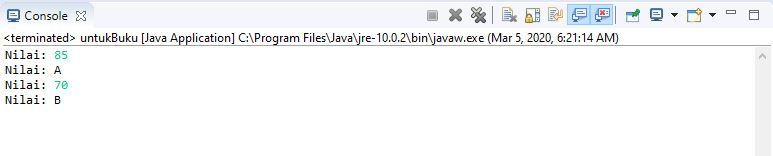
\includegraphics[scale=0.6]{pictures/hasil_if_else.jpg}
    \caption{Hasil program if else}
    \label{}
\end{figure}

\newpage
\subsection{Percabangan IF/ELSE/IF}
\begin{figure}[h!]
    \centering
    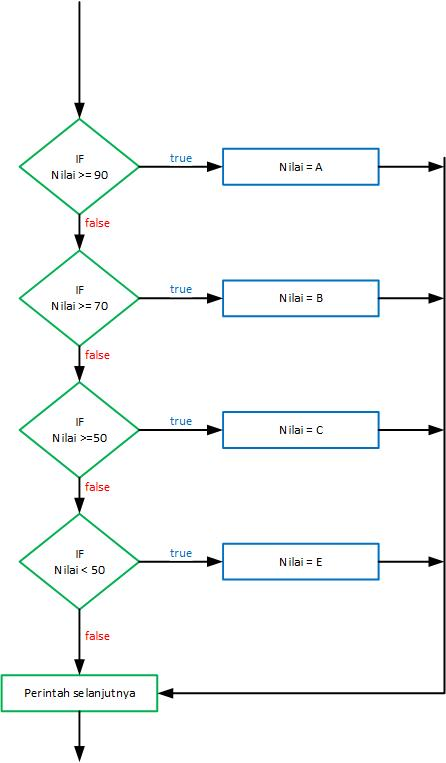
\includegraphics[scale=0.5]{pictures/flowmap_if_else_if.jpg}
    \caption{Flowmap logika IF/ELSE/IF}
    \label{}
\end{figure}

Jika kita lihat pada percabangan IF/ELSE hanya memiliki dua percabangan saja yaitu jika kondisi true dan false. Namun  pada percabangan IF/ELSE/IF, percabangan bisa memiliki banyak pilihan ketika kondisi yang dijalankan memiliki nilai false.

Struktur dari IF/ELSE/IF:
\begin{lstlisting}[language=Java]
if (statement 0) {
    // maka kerjakan perintah ini
    // perintah 1
    // perintah 2
    // ....
} else if (statement 1) {
    // kerjakan perintah ini
    // perintah 1
    // perintah 2
    // ....
} else if (statement 2) {
    // kerjakan perintah ini
    // perintah 1 juga
    // perintah 2 juga 
    // ....
} esle {
    // kerjakan perintah ini
    // hanya jika 
    // kondisi statement diatas tidak ada yang benar
    // ....
}    
\end{lstlisting}

\noindent\fcolorbox{red}{yellow}{%
    \minipage[b]{\dimexpr\linewidth\fboxsep\fboxrule\relax}
    Contoh dalam kegiatan sehari - hari adalah ketika dosen akan menentukan nilai grade dari mahasiswa. Jika Nilai >= 90 maka Grade = A, jika Nilai >= 70 maka Grade = B, jika Nilai >= 50 Grade C dan nilai < 50 maka Grade E.
    \endminipage}

\medskip

Bentuk contoh tersebut jika diubah menjadi bahasa program:
\begin{lstlisting}[language=Java]
public static void main(String[] args) {

    // membuat variabel Nilai dan scanner
    int nilai = 0;
    String grade;
        
    Scanner scan = new Scanner(System.in);

    // mengambil input
    System.out.print("Nilai: ");
        nilai = scan.nextInt();

    // IF/ELSE/IF untuk menentukan grade nilai mahasiswa 
    if ( nilai >= 90 ) {
        grade = "A";
    } else if ( nilai >= 70 ){
        grade = "B";
    } else if ( nilai >= 50 ){
        grade = "C";
    } else {
        grade = "E";
    }

    // Mencetak Grade dai nilai yang sudah diinputkan 
    System.out.println("Grade: " + grade);

}
\end{lstlisting}

Hasil dari program yang dijalankan adalah:
\begin{figure}[h!]
    \centering
    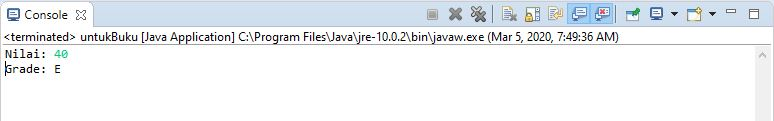
\includegraphics[scale=0.6]{pictures/hasil_if_else_if.JPG}
    \caption{Hasil program IF/ELSE/IF}
    \label{}
\end{figure}

\newpage
\subsection{Percabangan SWITCH/CASE}
\begin{figure}[h!]
    \centering
    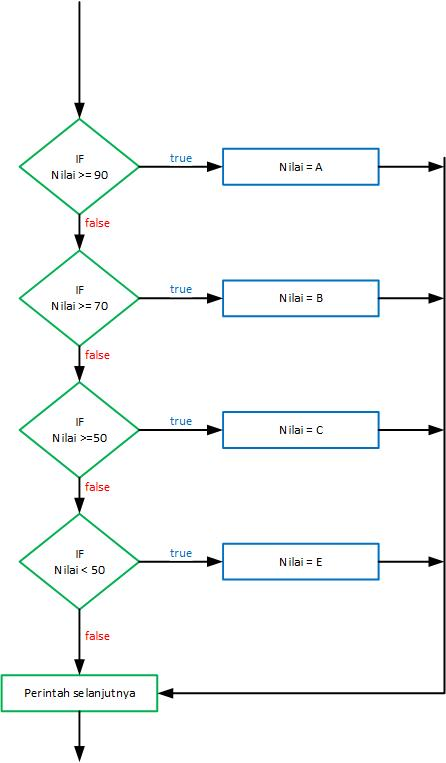
\includegraphics[scale=0.5]{pictures/flowmap_if_else_if.jpg}
    \caption{Flowmap logika SWITCH/CASE}
    \label{}
\end{figure}
Percabangan SWITCH/CASE secara fungsi hampir sama dengan percabangan IF/ELSE/IF namun pada percabangan ini perlu diingat bahwa kata kunci yang digunakan adalah \textcolor{pred}{switch} dan \textcolor{pred}{case}.

Bentuk program dari SWITCH/CASE adalah:
\begin{lstlisting}[language=Java]
switch(variabel){
    case 1:
        // Kerjakan perintah ini
        // perintah ini juga
        // perintah ini
        // ...
        break;
    case 2:
        // Kerjakan perintah ini
        // perintah ini juga
        // perintah ini
        // ...
        break;
    case 3:
        // Kerjakan perintah ini
        // perintah ini juga
        // perintah ini
        // ...
        break;
    default:
        // Kerjakan perintah ini
        // perintah ini juga
        // perintah ini
        // ...
	break;
}
\end{lstlisting}
Case 1 disini berisi Variabel yang akan dibandingkan sehingga memiliki hasil akhir true tau false.

\medskip

\noindent\fcolorbox{red}{yellow}{%
    \minipage[b]{\dimexpr\linewidth\fboxsep\fboxrule\relax}
    Contoh dalam kegiatan sehari - hari adalah ketika anda memiliki banyak pilihan seperti pada mesin ATM. Pada mesin ini disediakan beberapa pilihan menu seperti transfer, tarik tunai, cek saldo, dan lain-lain.
    \endminipage}

\medskip

Bentuk contoh tersebut jika diubah menjadi bahasa program:
\begin{lstlisting}[language = Java]
// membuat variabel dan Scanner
String pilihan;
Scanner scan = new Scanner(System.in);

// mengambil input
System.out.println("Selamat Datang di atm SNI");
System.out.println("1. Cek Saldo");
System.out.println("2. Tarik Tunai");
System.out.println("3. Setor");
System.out.println("Pilih Menu: ");
pilihan = scan.nextLine();

switch(pilihan){
    case "1":
        System.out.println("Saldo anda Rp.0,-");
        break;
    case "2":
        System.out.println("Anda Tidak Punya Saldo");
        break;
    case "3":
        System.out.println("Setor trosss");
        break;
    default:
        System.out.println("Masukan pilihan dengan benar!");
}
\end{lstlisting}

Hasil dari program yang dijalankan: 
\begin{figure}[h!]
    \centering
    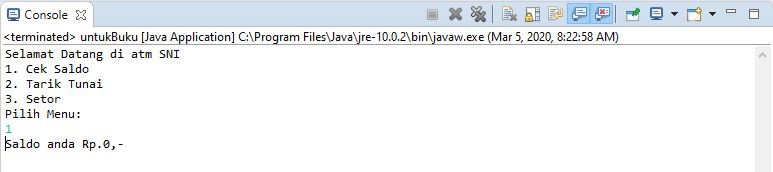
\includegraphics[scale=0.6]{pictures/hasil_switch_case.JPG}
    \caption{Hasil program SWITCH/CASE}
    \label{}
\end{figure}

\newpage
\subsection{Percabangan dalam percabangan (\textit{Nested})}
\begin{figure}[h!]
    \centering
    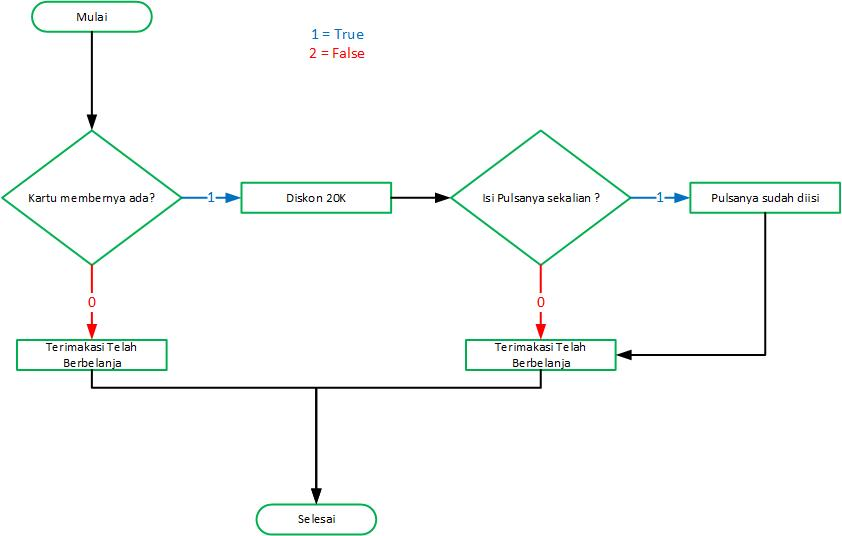
\includegraphics[scale=0.5]{pictures/flowmap_percabangan_dalam_percabangan.jpg}
    \caption{Flowmap logika percabangan dalam percabangan}
    \label{}
\end{figure}
Pada dasarnya percabangan dalam percabangan ini hampir sama dengan IF/ELSE karena menggunakanperintah \textcolor{pred}{if} dan \textcolor{pred}{else}. Namun ada if/else dalam if/else sehingga disebut "Percabangan dalam percabangan (\textit{Nested})"

Strukrur percabangan dalam percabangan:
\begin{lstlisting}[language=Java]
if (statement) {
        if (statement) {
            // Eksekusi perintah ini
            // Perintah ini
            // perintah itu
            // ....
        } else if (statement2) {
            // Eksekusi perintah ini
            // Perintah ini
            // perintah itu
            // ....
        } else {
            // Eksekusi perintah ini
            // Perintah ini
            // perintah itu
            // ....
        }

    } else {
        if (statement) {
            // Eksekusi perintah ini
            // Perintah ini
            // perintah itu
            // ....
        } else {
            // Eksekusi perintah ini
            // Perintah ini
            // perintah itu
            // ....
        }
    }
\end{lstlisting}

\medskip

\noindent\fcolorbox{red}{yellow}{%
    \minipage[b]{\dimexpr\linewidth\fboxsep\fboxrule\relax}
    Contoh dalam kegiatan sehari - hari adalah ketika membeli sesuatu di minimarket, kemudian kasir bertanya kartu member. Jika memiliki kartu member maka diskon 20.000 dan kasir akan bertanya lagi apakah akan isi pulsa sekalian? jika ya maka pulsa diisi, jika tidak maka selesai. Sedangkan jika tidak punya kartu member, Maka proses langsung selesai.
    \endminipage}

\medskip

Bentuk Contoh tersebut jika diubah menjadi bahasa program:
\begin{lstlisting}[language=Java]
// deklarasi variabel dan Scanner
String kartu, pulsa;
Scanner scan = new Scanner(System.in);

// mengambil input
System.out.print("Apakah ada kartu membernya?: ");
kartu = scan.nextLine();

// proses
if (kartu.equalsIgnoreCase("ya")) {
    System.out.println("Anda mendapat diskon 20.000");
    System.out.print("Mau isi pulsa sekalian?: ");
    pulsa = scan.nextLine();
    if (pulsa.equalsIgnoreCase("ya")) {
        System.out.println("Pulsa Terisi");
        System.out.println("Terimakasih telah berbelanja");
    } else if (pulsa.equalsIgnoreCase("tidak")) {
        System.out.println("Terimakasih telah berbelanja");
    } else {
        System.out.println("Terimakasih telah berbelanja");
    }

} else {
    System.out.println("Terimakasih telah berbelanja");
}
\end{lstlisting}

Hasil dari program yang dijalankan:
\begin{figure}[h!]
    \centering
    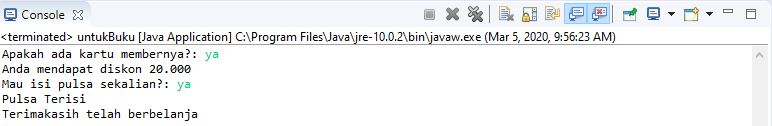
\includegraphics[scale=0.6]{pictures/hasil_percabangan_dalam_percabangan.JPG}
    \caption{Hasil program percabangan dalam percabangan}
    \label{}
\end{figure}










\chapter{Java Development Kit}
\section{JDK \textit{Java Development Kit}}
Java Development Kit (JDK) adalah salah satu dari tiga package inti yang digunakan dalam pemrograman Java, bersama dengan JVM (Java Virtual Machine) dan JRE (Java Runtime Environment)..\cite{webjavaworld1}

%\begin{references}{Ham62}
%\bibitem[Kil76]{kilb}J. S. Kilby,
%``Invention of the Integrated Circuit,'' {\it IEEE Trans. Electron Devices,}
%{\bf ED-23,} 648 (1976).
%
%\bibitem[Ham62]{hamm}R. W. Hamming,
%                 {\it Numerical Methods for Scientists and 
%                 Engineers}, Chapter N-1, McGraw-Hill, 
%                 New York, 1962.
%
%\bibitem[Hu86]{lee}J. Lee, K. Mayaram, and C. Hu, ``A Theoretical
%               Study of Gate/Drain Offset in LDD MOSFETs''
%                     {\it IEEE Electron Device Lett.,} {\bf EDL-7}(3). 152 
%                     (1986).
%
%\bibitem[Ber87]{berm}A. Berenbaum, 
%B. W. Colbry, D.R. Ditzel, R. D Freeman, and 
%K.J. O'Connor, ``A Pipelined 32b Microprocessor with 13 kb of Cache Memory,''
%{it Int. Solid State Circuit Conf., Dig. Tech. Pap.,} p. 34 (1987).
%
%\end{references}


\bibliographystyle{IEEEtran} 
%\def\bibfont{\normalsize}
\bibliography{referensi}


%%%%%%%%%%%%%%%
%%  The default LaTeX Index
%%  Don't need to add any commands before \begin{document}
\printindex

%%%% Making an index
%% 
%% 1. Make index entries, don't leave any spaces so that they
%% will be sorted correctly.
%% 
%% \index{term}
%% \index{term!subterm}
%% \index{term!subterm!subsubterm}
%% 
%% 2. Run LaTeX several times to produce <filename>.idx
%% 
%% 3. On command line, type  makeindx <filename> which
%% will produce <filename>.ind 
%% 
%% 4. Type \printindex to make the index appear in your book.
%% 
%% 5. If you would like to edit <filename>.ind 
%% you may do so. See docs.pdf for more information.
%% 
%%%%%%%%%%%%%%%%%%%%%%%%%%%%%%

%%%%%%%%%%%%%% Making Multiple Indices %%%%%%%%%%%%%%%%
%% 1. 
%% \usepackage{multind}
%% \makeindex{book}
%% \makeindex{authors}
%% \begin{document}
%% 
%% 2.
%% % add index terms to your book, ie,
%% \index{book}{A term to go to the topic index}
%% \index{authors}{Put this author in the author index}
%% 
%% \index{book}{Cows}
%% \index{book}{Cows!Jersey}
%% \index{book}{Cows!Jersey!Brown}
%% 
%% \index{author}{Douglas Adams}
%% \index{author}{Boethius}
%% \index{author}{Mark Twain}
%% 
%% 3. On command line type 
%% makeindex topic 
%% makeindex authors
%% 
%% 4.
%% this is a Wiley command to make the indices print:
%% \multiprintindex{book}{Topic index}
%% \multiprintindex{authors}{Author index}

\end{document}

